diff --git a/manuscript.tex b/manuscript.tex
index 0cb5340..a9773d2 100644
--- a/manuscript.tex
+++ b/manuscript.tex
@@ -1,5 +1,6 @@
-\documentclass[fleqn]{IJCAS}  % Comment this line out if you need a4paper
+\documentclass[10pt,fleqn]{IJCAS}  % Comment this line out if you need a4paper
 \usepackage{ijcas_packages}
+\allowdisplaybreaks[1]
 
 \newcommand{\squeezeup}{\vspace{-2.5mm}}
 
@@ -33,7 +34,7 @@ The effectiveness of the proposed control system is demonstrated through numeric
 %%%%%%%%%%%%%%%%%%%%%%%%%%%%%%%%%%%%%%%%%%%%%%%%%%%%%%%%%%%%%%%%%%%%%%%%%%%%%%%%
 
 \begin{keywords}
-attitude control, asymptotic stability, special orthogonal group, constraint
+adaptive control, attitude control, constraint, obstacle, special orthogonal group
 %At least four key words or phrases in alphabetical order, separated by commas.
 \end{keywords}
 
@@ -116,7 +117,7 @@ Artificial potential functions are commonly used to handle kinematic constraints
 The goal is the design of attractive and repulsive terms which drive the system toward or away from a certain obstacle, respectively.
 The attractive function is designed to drive the system towards the desired state.
 Similarly, a repulsive function is constructed such that the system is directed away from the constraints. 
-The superposition of the these functions allows one to apply standard feedback control schemes for stabilization and tracking.
+The superposition of these functions allows one to apply standard feedback control schemes for stabilization and tracking.
 More specifically, artificial potential functions have previously been applied to the spacecraft attitude control problem in~\cite{lee2011b,mcinnes1994}.
 However, both of these approaches were developed using attitude parameterizations, namely Euler angles and quaternions, and as such, they are limited by the singularities of minimal representations or the ambiguity of quaternions.
 
@@ -173,9 +174,11 @@ More explicitly,
 \end{align*}
 for $x=[x_1,x_2,x_3]^T\in\R^{3}$. 
 The inverse of the hat map is denoted by the \textit{vee} map $\vee:\so\rightarrow\R^{3}$. 
+We use the notation \( \hat{x}\) and \( \parenth{x}^\wedge\) interchangeably.
+In particular, we use the latter form when the expression for the argument of the \textit{hat} map is long. 
 Several properties of the hat map are summarized as
 \begin{gather}
-   % \hat x y = x\times y = - y\times x = - \hat y x,\\
+   \hat x y = x\times y = - y\times x = - \hat y x, \label{eqn:cross_product}\\
     x\cdot \hat y z = y\cdot \hat z x,\quad \hat x\hat y z = (x\cdot z) y - (x\cdot y ) z\label{eqn:STP},\\
    % \hat x\hat y z = (x\cdot z) y - (x\cdot y ) z,\label{eqn:VTP}\\
    % C^TC=-C^T\hat e_3^2 C = I_2
@@ -208,7 +211,7 @@ We formulate this hard constraint as
 where we assume \( \ang{0} \leq \theta \leq \ang{90}  \) is the required minimum angular separation between \( r \) and \( R^T v \). 
 The objective is to a determine a control input \( u \) that stabilizes the system from an initial attitude \( R_0 \) to a desired attitude \( R_d \) while ensuring that~\cref{eqn:constraint} is always satisfied.
 \squeezeup
-\section{Attitude Control on $\SO$ with Inequality Constraints}
+\section{Attitude Control on $\SO$ with Inequality Constraints}\label{sec:attitude_control}
 
 The first step in designing a control system on a nonlinear manifold \( \Q \) is the selection of a proper configuration error function. 
 This configuration error function, \( \Psi : \Q \times \Q \to \R \), is a smooth and proper positive definite function that measures the error between the current configuration and a desired configuration. 
@@ -226,13 +229,13 @@ The proposed attitude configuration error function and several properties are su
 %We assume a desired attitude command \( ( R_d, \Omega_d = 0 ) \), the current attitude and angular velocity \( ( R, \Omega) \), and a state constraint~\cref{eqn:constraint} are given.
 Define an attitude error function \( \Psi : \SO \to \R \), an attitude error vector \( e_R \in \R^3 \), and an angular velocity error vector \( e_\Omega \in \R^3 \) as follows:
 \begin{gather}
-	\Psi(R) = A(R) B(R) , \label{eqn:psi} \\
-	e_R = e_{R_A} B(R) + A(R) e_{R_B} , \label{eqn:eR} \\
+	\Psi(R, R_d) = A(R, R_d) B(R) , \label{eqn:psi} \\
+	e_R = e_{R_A} B(R) + A(R,R_d) e_{R_B} , \label{eqn:eR} \\
 	e_\Omega = \Omega , \label{eqn:eW}
 \end{gather}
 with
 \begin{gather}
-	A(R) = \frac{1}{2} \tr{G \left( I - R_d^T R\right)} , \label{eqn:A} \\
+	A(R,R_d) = \frac{1}{2} \tr{G \left( I - R_d^T R\right)} , \label{eqn:A} \\
 	B(R) = 1 - \frac{1}{\alpha} \ln \left( \frac{\cos \theta -  r^T R^T v}{1 + \cos \theta}\right) . \label{eqn:B} \\
 	e_{R_A} = \frac{1}{2} \parenth{G R_d^T R - R^T R_d G} ^ \vee , \label{eqn:eRA} \\
 	e_{R_B} = \frac{ \left( R^T v\right)^\wedge r}{\alpha \left(r^T R^T v - \cos \theta \right)} . \label{eqn:eRB} 
@@ -242,13 +245,15 @@ Then, the following properties hold
 \begin{enumerate}[(i)]
 	\item \label{item:prop_psi_psd} \(\Psi\) is positive definite about \( R = R_d\) on $\SO$.
 	\item \label{item:prop_era}The variation of \( A(R) \) with respect to a variation of \( \delta R = R \hat{\eta} \) for \( \eta \in \R^3 \) is given by
-	\begin{align}
-		\dirDiff{A}{R} &= \eta \cdot e_{R_A} .
+	\begin{align}\label{eq:dirDiff_A}
+		\dirDiff{A}{R} &= \eta \cdot e_{R_A} ,
 	\end{align}
+	where the notation \( \dirDiff{A}{R} \) represents the directional derivative of $A$ with respect to $R$ along $\delta R$.
 	\item \label{item:prop_erb} The variation of \( B(R) \) with respect to a variation of \( \delta R = R \hat{\eta} \) for \( \eta \in \R^3 \) is given by
-	\begin{align}
-		\dirDiff{B}{R} &= \eta \cdot e_{R_{B}} .
+	\begin{align}\label{eq:dirDiff_B}
+		\dirDiff{B}{R} &= \eta \cdot e_{R_{B}}.
 	\end{align}
+%    where the notation \( \D_R A \) and \(\D_R B\) represents the derivative of \( A \) or \( B \) with respect to \( R\).
 %	\item \label{item:prop_crit}The error function \( \Psi \) is minimized when \(R = R_d\).
 	\item \label{item:prop_era_upbound}An upper bound of \( \norm{e_{R_A}} \) is given as:
 	\begin{align}
@@ -260,6 +265,15 @@ Then, the following properties hold
 		h_2 &= \min\braces{\parenth{g_1 -g_2}^2,\parenth{g_2 -g_3}^2 , \parenth{g_3 -g_1}^2} ,\\
 		h_3 &= \min\braces{\parenth{g_1 + g_2}^2, \parenth{g_2 + g_3}^2 , \parenth{g_3 + g_1}^2}.		
 	\end{align*}
+    \item \label{item:prop_psi_quadratic} \( \Psi \) is a locally quadratic function, which means there exist constants \( 0 < n_1 \leq n_2 \) such that
+    \begin{align}\label{eq:psi_bound}
+        n_1 \norm{e_R}^2 \leq \Psi(R) \leq n_2 \norm{e_R}^2 ,
+    \end{align}
+    on the neighborhood $D$ of the desired attitude \( R_d \)
+    \begin{align}\label{eq:psi_quadratic_domain}
+        D = \braces{R\in\SO  \vert \Psi < \psi < h_1, r^T R^T v < \beta < \cos \theta}
+    \end{align}
+    for $0<\psi < h_1 $ and $0< \beta<\cos\theta$. 
 \end{enumerate}
 \end{prop}
 \begin{proof}
@@ -271,24 +285,27 @@ In order to visualize the attitude error function on \( \SO \), we utilize a sph
 Recall, that the spherical coordinate system represents the position of a point relative to an origin in terms of a radial distance, azimuth, and elevation.
 This coordinate system is commonly used to define locations on the Earth in terms of a latitude and longitude.
 Similarly, the positions of celestial objects are defined on the celestial sphere in terms of right ascension and declination. 
+\end{multicols}
 \begin{figure}[H]%
     \centering 
-    \subfigure[Attractive \( A(R) \) \label{fig:attract_error}]{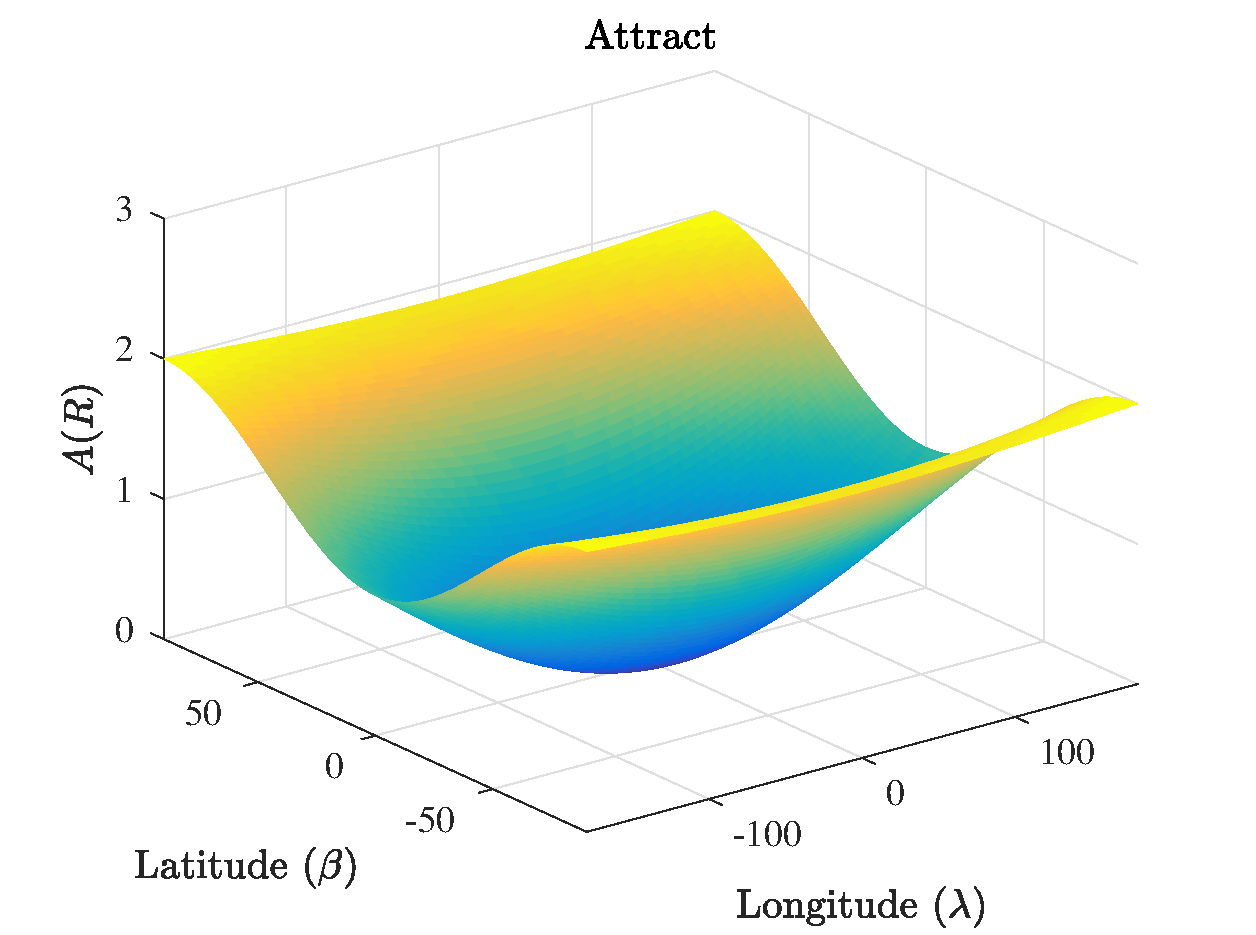
\includegraphics[width=0.45\columnwidth]{attract_error} }~
-    \subfigure[Repulsive \( B(R) \) \label{fig:avoid_error} ]{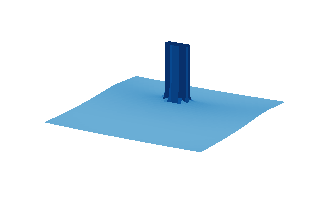
\includegraphics[width=0.45\columnwidth]{avoid_error} }\\%add desired spacing between images, e. g. ~, \quad, \qquad, \hfill etc. %(or a blank line to force the subfigure onto a new line) 
-    \subfigure[Configuration \( \Psi \) \label{fig:combined_error}]{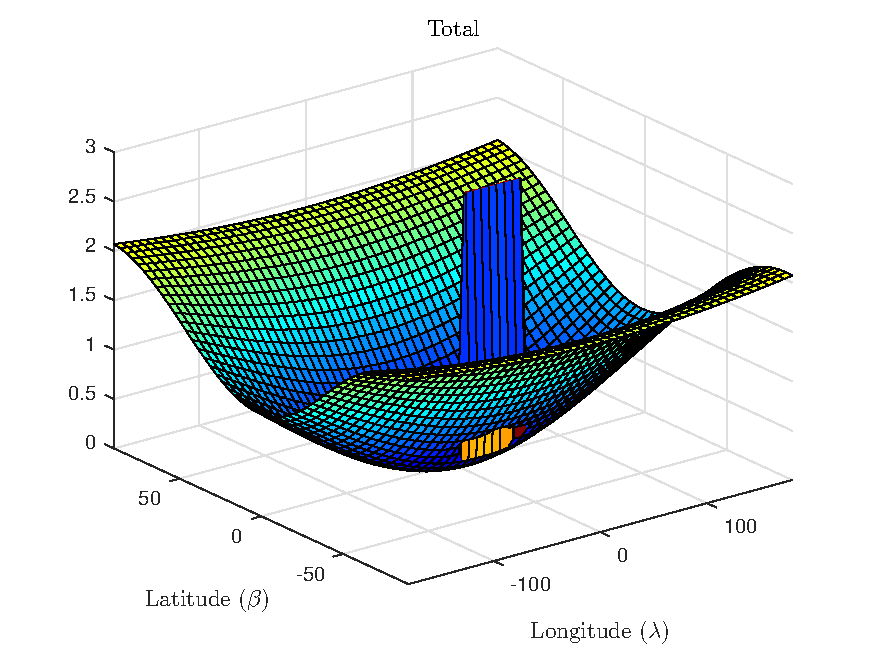
\includegraphics[width=0.45\columnwidth]{combined_error} }%
-    \caption{Configuration error function visualization}
+    \subfigure[Attractive \( A(R) \) \label{fig:attract_error}]{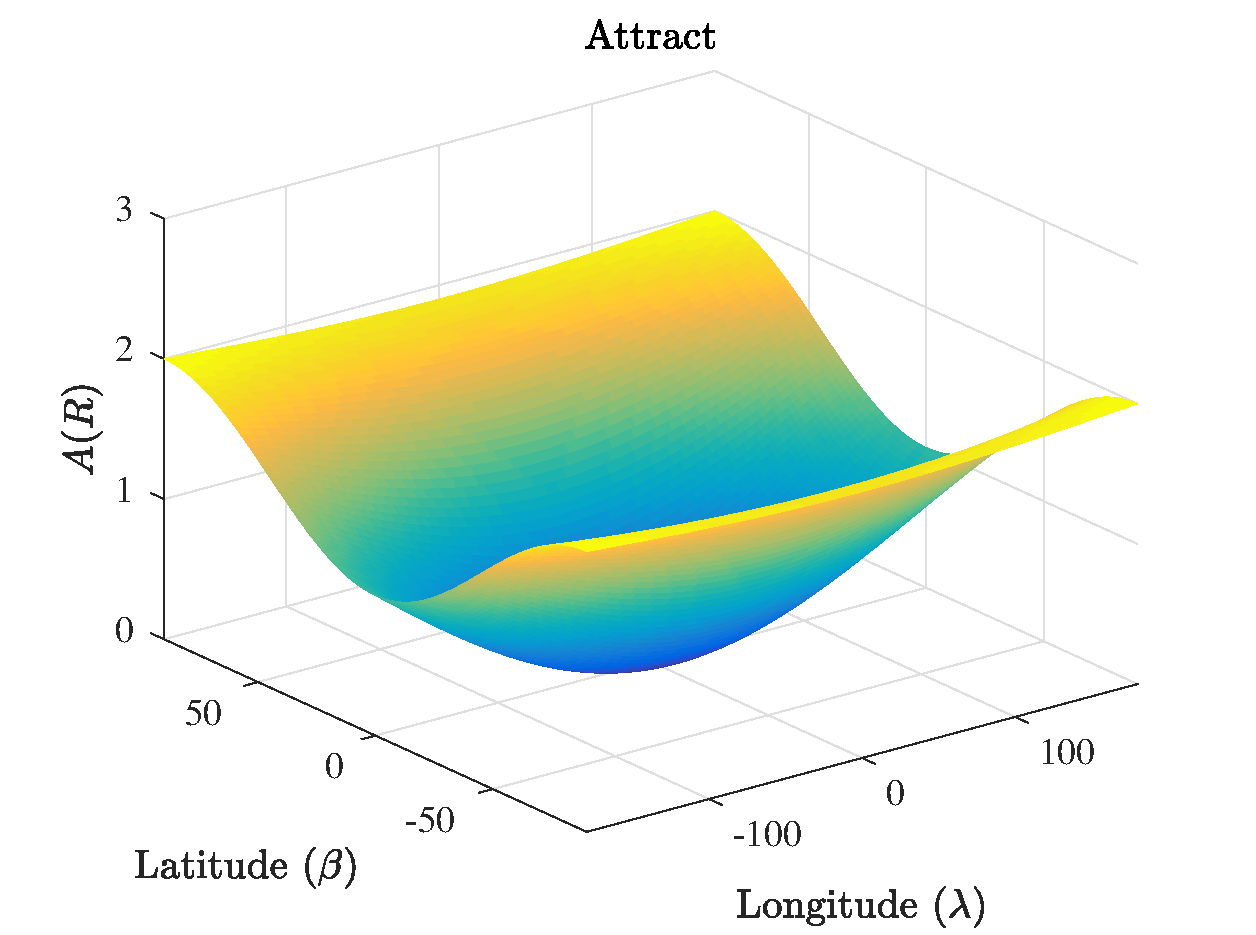
\includegraphics[width=0.33\columnwidth]{attract_error} }~
+    \subfigure[Repulsive \( B(R) \) \label{fig:avoid_error} ]{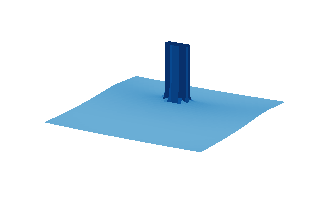
\includegraphics[width=0.33\columnwidth]{avoid_error} }~
+    \subfigure[Combined \( \Psi \) \label{fig:combined_error}]{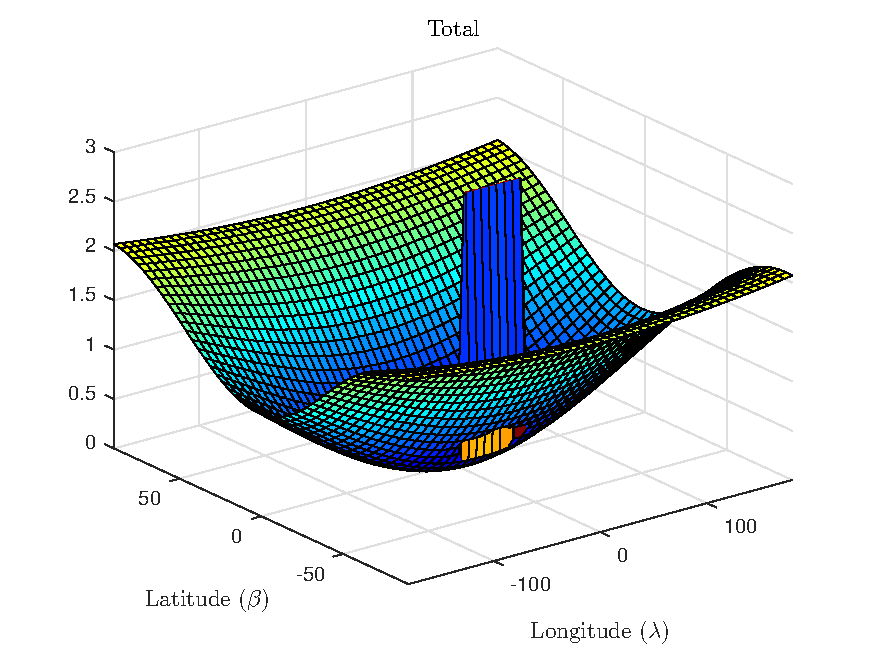
\includegraphics[width=0.33\columnwidth]{combined_error} }%
+    \caption{Visualization of Configuration Error Functions using spherical coordinate representation}
     \label{fig:config_error} 
 \end{figure}%
+\begin{multicols}{2}
 We apply this concept and parametrize the rotation matrix \( R \in \SO \) in terms of the spherical angles \( \SI{-180}{\degree} \leq \lambda \leq \SI{180}{\degree}  \) and \( \SI{-90}{\degree} \leq \beta \leq \SI{90}{\degree} \). 
 Using the elementary Euler rotations, the rotation matrix is now defined as \( R = \exp( \lambda \hat{e}_2) \exp( \beta \hat{e}_3) \).
 We iterate over the domains of \( \lambda\) and \(\beta\) in order to rotate the body-fixed vector \( r \) throughout the two-sphere \( \S^2 \).
 Applying this method,~\cref{fig:config_error} allows us to visualize the error function on \( \SO \).
+The horizontal axes of~\cref{fig:config_error} represent the domain of the spherical angles \( \lambda \) and \( \beta \) in degrees, while the vertical axes represent the unitless magnitude of the error functions defined in~\cref{eqn:psi,eqn:A,eqn:B}.
 The attractive error function, given by~\cref{eqn:A}, has been previously used for attitude control on \(\SO\).
 The potential well of \( A(R)\) is illustrated in~\cref{fig:attract_error}, where the desired attitude lies at the minimum of \( A(R) \).
 
 To incorporate the state inequality constraints we apply a logarithmic barrier term.
 Barrier functions are typically used in optimal control and motion planning applications.
-A visualization of the configuration error function is presented in~\cref{fig:avoid_error} which shows that as the boundary of the constraint is neared, or \( r^T R^T v \to \cos \theta \), the barrier term increases, \( B \to \infty\).
+A visualization of the repulsive error function is presented in~\cref{fig:avoid_error} which shows that as the boundary of the constraint is neared, or \( r^T R^T v \to \cos \theta \), the barrier term increases, \( B \to \infty\).
 We use the scale factor~\(\frac{1}{1+\cos \theta} \) to ensure that \( \Psi \) remains positive definite.
 The logarithmic function is popular as it quickly decays away from the constraint boundary.
 The positive constant \( \alpha \) serves to shape the barrier function.
@@ -306,10 +323,10 @@ We present the dynamics of the configuration error function in~\Cref{prop:error_
 	The attitude error dynamics for \( \Psi, e_R, e_\Omega \) satisfy 
 	\begin{gather}
 		\diff{}{t} \parenth{\Psi} = e_R \cdot e_\Omega , \label{eqn:psi_dot}\\
-		\diff{}{t} \parenth{e_R} = \dot{e}_{R_A} B(R) + e_{R_A} \dot{B}(R) + \dot{A}(R)e_{R_B} + A \dot{e}_{R_B} , \label{eqn:eR_dot}\\
+		\diff{}{t} \parenth{e_R} = \dot{e}_{R_A} B + e_{R_A} \dot{B} + \dot{A}e_{R_B} + A \dot{e}_{R_B} , \label{eqn:eR_dot} \\
 		\diff{}{t} \parenth{e_{R_A}} = E(R, R_d) e_\Omega , \label{eqn:eRA_dot} \\
 		\diff{}{t} \parenth{e_{R_B}} = F(R) e_\Omega , \label{eqn:eRB_dot} \\
-		\diff{}{t} \parenth{A(R)} = e_{R_A} \cdot e_\Omega , \label{eqn:A_dot} \\
+    	\diff{}{t} \parenth{A(R)} = e_{R_A} \cdot e_\Omega , \label{eqn:A_dot} \\
 		\diff{}{t} \parenth{B(R)} = e_{R_B} \cdot e_\Omega , \label{eqn:B_dot} \\
 		\diff{}{t} \parenth{e_\Omega} = J^{-1} \parenth{-\Omega \times J \Omega + u + W(R, \Omega) \Delta} , \label{eqn:eW_dot}
 	\end{gather}
@@ -326,7 +343,7 @@ See~\Cref{proof:error_dyn}
 
 \subsection{Attitude Control without Disturbance}
 We introduce a nonlinear geometric controller for the attitude stabilization of a rigid body.
-We first assume that there is no disturbance, i.e., \( \Delta = 0 \) and present a nonlinear controller in~\Cref{prop:att_control}.
+We first assume that there is no disturbance, i.e., \( \Delta = 0 \), and present a nonlinear controller in~\Cref{prop:att_control}.
 \begin{prop}[Attitude Control]\label{prop:att_control}
 	Given a desired attitude command \( \parenth{R_d, \Omega_d = 0} \), which satisfies the constraint~\cref{eqn:constraint}, and positive constants \( k_R, k_\Omega \in \R \) we define a control input \( u \in \R^3 \) as follows
 	\begin{gather}
@@ -347,16 +364,17 @@ Aerial vehicles will similarly experience external torques due to air currents o
 An adaptive control system is introduced to asymptotically stabilize the system to a desired attitude while ensuring that state constraints are satisfied. %We first show several properties of the controlled system. 
 
 \begin{prop}[Bound on \( \bm{\dot{e}_R} \)]\label{prop:eR_dot_bound}
-Consider a domain \( D \) about the desired attitude defined as
-\begin{align}
-	D = \braces{R \in \SO \vert \Psi < \psi < h_1, r^T R^T v < \beta < \cos \theta}. \label{eqn:domain}
-\end{align}
-Then the following statements hold:
+Consider the neighborhood \( D \), given in~\cref{prop:config_error}, about the desired attitude, then the following statements hold:
 \begin{enumerate}[(i)]
 	\item \label{item:prop_eR_dot_bound_AB} Upper bounds of \( A(R) \) and \( B(R) \) are given by
 	\begin{gather}
-		\norm{A} < c_A  , \quad \norm{B} < c_B . \label{eqn:AB_bound}
+		\norm{A} < b_2 \norm{e_{R_A}}^2 < c_A  , \quad \norm{B} < c_B . \label{eqn:AB_bound}
 	\end{gather}
+  where the constant \( b_2\) is given by \( b_2 = \frac{h_1 h_4}{h_5 \parenth{h_1 - \psi}}\) for
+  \begin{align*}
+    h_4 &= \min\braces{g_1 + g_2, g_2 + g_3 , g_3 + g_1} ,\\
+    h_5 &= \min\braces{\parenth{g_1 + g_2}^2,\parenth{g_2 + g_3}^2 , \parenth{g_3 + g_1}^2} .\\
+  \end{align*}
 	\item \label{item:prop_eR_dot_bound_EF} Upper bounds of \( E(R,R_d) \) and \( F(R) \) are given by
 	\begin{gather}
 		\norm{E} \leq \frac{1}{\sqrt{2}} \tr{G}  , \label{eqn:E_bound} \\
@@ -367,6 +385,7 @@ Then the following statements hold:
 		\norm{e_{R_A}} \leq \sqrt{\frac{\psi}{b_1}}, \label{eqn:eRA_bound} \\
 		\norm{e_{R_B}} \leq \frac{\sin\theta}{\alpha \parenth{\cos \theta - \beta}}. \label{eqn:eRB_bound}
 	\end{gather}
+
 \end{enumerate}
 These results are combined to yield a maximum upper bound of the time derivative of the attitude error vector \( \dot{e}_R \) as
 \begin{gather}
@@ -392,9 +411,11 @@ Given  a desired attitude command \( (R_d, \Omega_d = 0 )\) and positive constan
 \end{align}
 If \( c \) is chosen such that
 \begin{gather}
-	0 < c < \frac{4 k_R k_\Omega}{k_\Omega^2 + 4 k-R \lambda_M H} , \label{eqn:c_bound}
+	0 < c < \min \braces{\sqrt{\frac{2 \lambda_m k_R n_1}{\lambda_M^2}},
+	%\sqrt{\frac{2 k_R n_2}{\lambda_M}}, 
+	\frac{4 k_R k_\Omega}{k_\Omega^2 + 4 k_R \lambda_M H}} , \label{eqn:c_bound}
 \end{gather}
-  the zero equilibrium of the error vectors is stable in the sense of Lyapunov. Furthermore, $e_R,e_\Omega\rightarrow 0$ as $t\rightarrow\infty$, and $\bar\Delta$ is uniformly bounded.
+  the zero equilibrium of the error vectors is stable in the sense of Lyapunov. Furthermore, $e_R,e_\Omega\rightarrow 0$ as $t\rightarrow\infty$, and $\bar\Delta$ is  bounded.
 \end{prop}
 \begin{proof}
 See~\Cref{proof:adaptive_control}
@@ -413,7 +434,18 @@ In addition, the rigorous mathematical proof guarantees stability.
 This is in contrast to many of the previous methods which offer no stability guarantees.
 The presented analysis offers provable bounds on the expected motion, which are critical for hardware implementation or mission critical applications.
 
-\section{Numerical Examples}
+\end{multicols}
+\begin{figure}[b]
+    \centering 
+    \subfigure[Attitude error vector \(e_R\) components \label{fig:eR_con}]{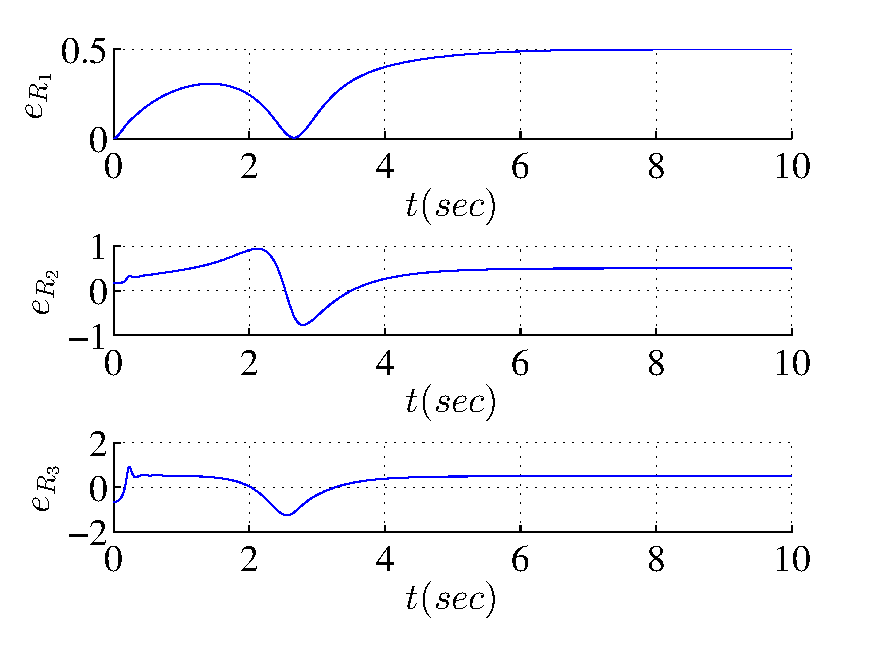
\includegraphics[width=0.3\columnwidth]{eR_con}  }~
+    \subfigure[Configuration error \( \Psi \) \label{fig:Psi_con}]{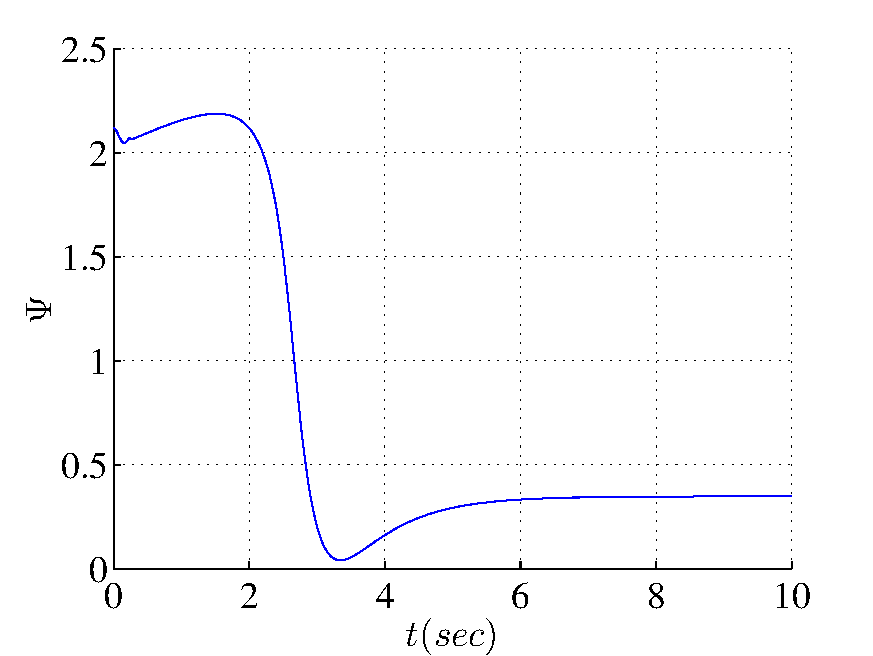
\includegraphics[width=0.3\columnwidth]{figures/Psi_con.pdf} }
+    \subfigure[Angle to each constraint \label{fig:con_angles_con}]{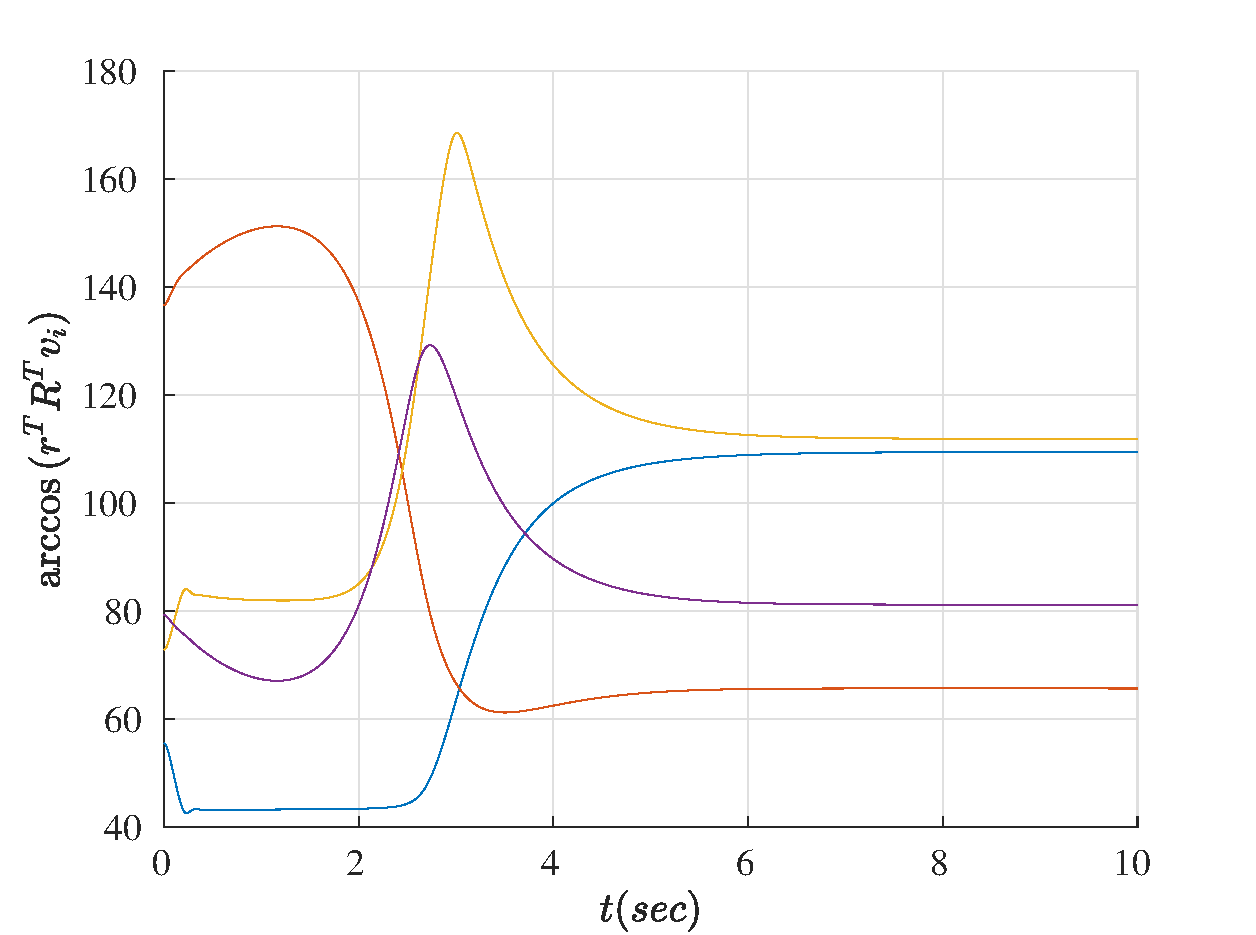
\includegraphics[width=0.3\columnwidth]{figures/constraint_angles_con.pdf} } 
+    \caption{Attitude stabilization without adaptive update law}
+    \label{fig:con} 
+\end{figure}
+\begin{multicols}{2}
+\section{Numerical Examples}\label{sec:numerical_simulation}
+
 We demonstrate the performance of the proposed control system via numerical simulation.
 The inertia tensor of a rigid body is given as
 \begin{gather*}
@@ -429,6 +461,15 @@ The control system parameters are chosen as
 	G = \text{diag} [0.9,1.1,1.0], \quad k_R = 0.4 , \quad	k_\Omega = 0.296 ,\\
 	c = 1.0 , \quad k_\Delta = 0.5 , \quad \alpha = 15 .
 \end{gather*}
+The diagonal matrix \( G \) serves as a weighting matrix for the relative difference between \( R \) and \( R_d \). 
+Using this term, the control designer can modify the shape of the attractive error function, given in~\cref{eqn:A}, and the resulting behavior of the closed loop system.
+Similarly, the constant \( \alpha \) is used to modify the shape of the repulsive error function, given in~\cref{eqn:B}.
+In general, this term is derived from the system design and the nature of the obstacles in the dynamic environment.
+For example, a system wishing to avoid pointing at a diffuse obstacle, such as incoming debris, may chose an appropriate value of \( \theta \), based on the best available information, and a relatively low \( \alpha \) to ensure additional safety margin near the constraint boundary. 
+Similarly, in an environment with several densely spaced obstacles, such as that presented in~\cref{fig:cad_adapt}, a much larger \( \alpha \) would enable more aggressive manuevers which pass closer to the constraint boundary without violation.
+This would increase the allowable region of operation in a highly constrained environment.
+The parameters \( k_R, k_\Omega, c, k_\Delta\) are control parameters used to modify the closed-loop behavior of the system.
+It is straightforward to chose \( k_R, k_\Omega, k_\Delta\), using a linear analysis, to satisfy desired response criteria, such as settling time or percent overshoot~\cite{nise2004}.
 A body fixed sensor is defined as \(r = [1,0,0]\), while multiple inequality constraints are defined in~\Cref{tab:constraints}.
 The simulation parameters are chosen to be similar to those found in~\cite{lee2011b}, however we increase the size of the constraint regions to create a more challenging scenario for the control system.
 \begin{table}[H]
@@ -444,41 +485,27 @@ Constraint Vector (\( v \)) & Angle (\( \theta \)) \\ \hline \hline
 
 The initial state is defined as \(R_0 =  \exp(\ang{225} \times \frac{\pi}{180} \hat{e}_3), \Omega_0 = 0\). 
 The desired state is \( R_d = I,\Omega_d = 0\).
-\begin{figure}[H] 
-    \centering 
-    \subfigure[Attitude error vector \(e_R\) \label{fig:eR_con}]{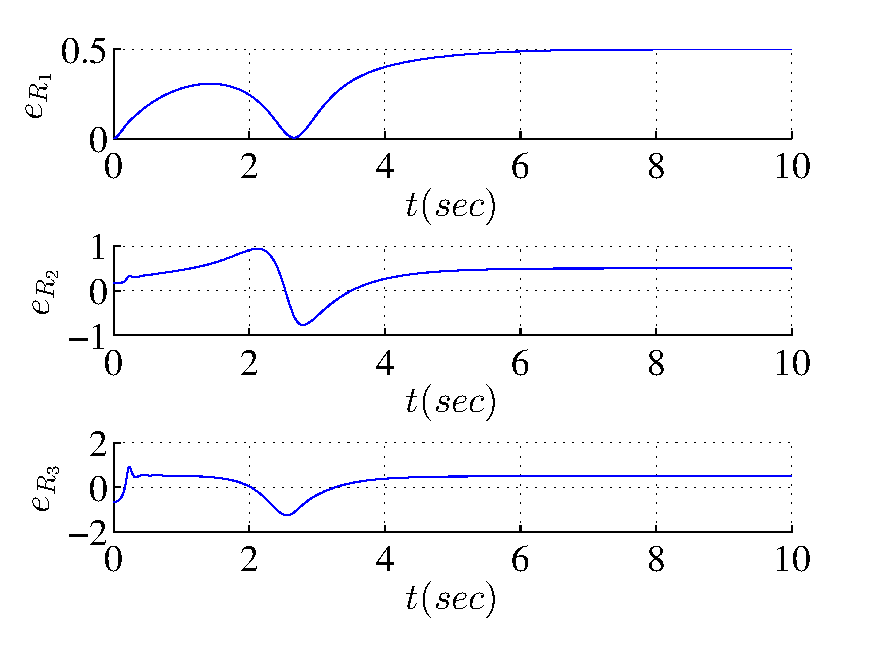
\includegraphics[width=0.5\columnwidth]{eR_con}  }~
-    \subfigure[Configuration error \( \Psi \) \label{fig:Psi_con}]{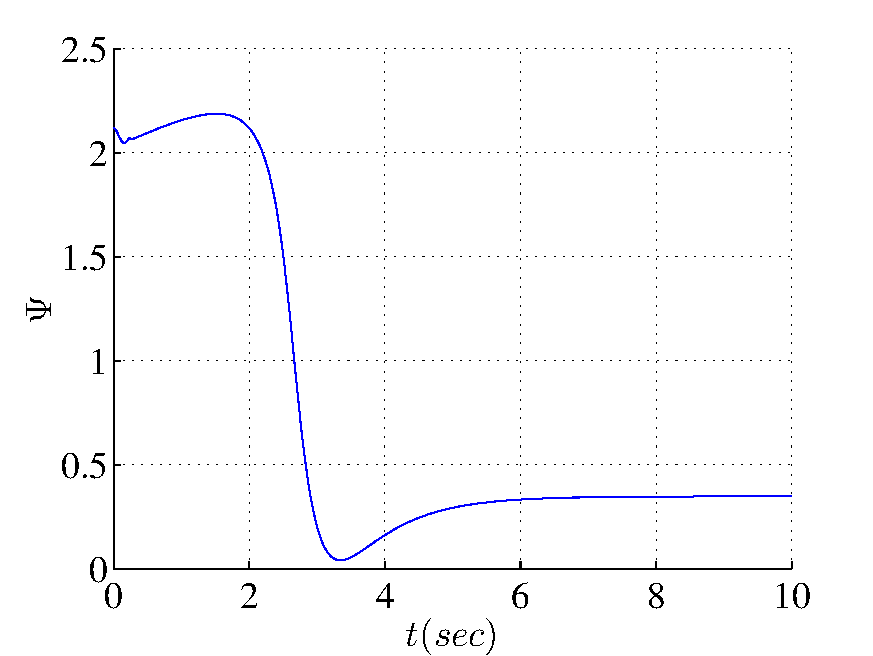
\includegraphics[width=0.5\columnwidth]{figures/Psi_con.pdf} }
-    \subfigure[Angle to constraints \label{fig:con_angles_con}]{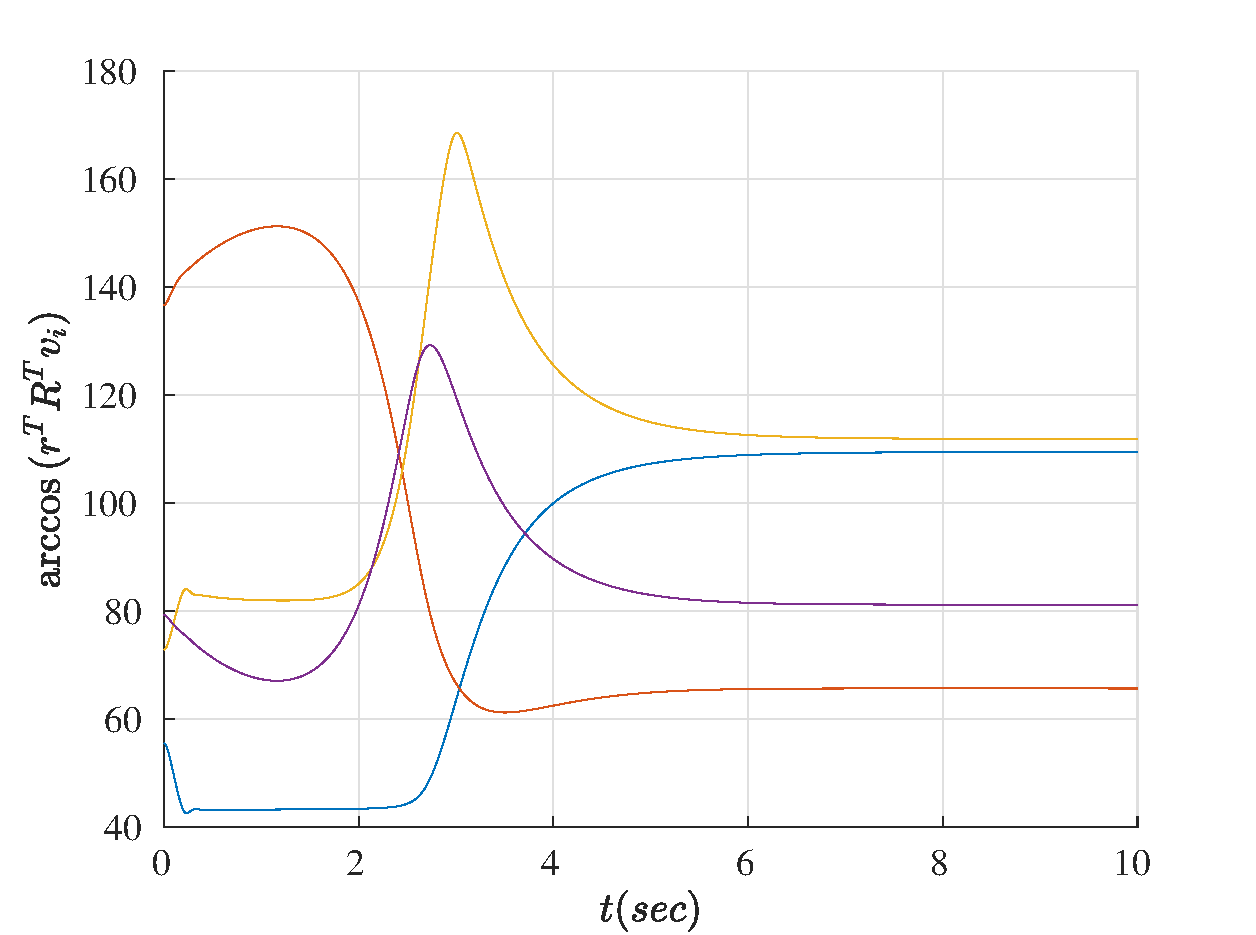
\includegraphics[width=0.5\columnwidth]{figures/constraint_angles_con.pdf} }  
-    \caption{Attitude stabilization without adaptive update law}
-    \label{fig:con} 
-\end{figure}
 We show simulation results for the system stabilizing about the desired attitude with and without the adaptive update law from~\Cref{prop:adaptive_control}.
-We assume a fixed disturbance of \(\Delta = \begin{bmatrix} 0.2 & 0.2 & 0.2 \end{bmatrix}^T \), with the function \( W(R,\Omega) = I \).
+We assume a fixed disturbance of \(\Delta = \begin{bmatrix} 0.2 & 0.2 & 0.2 \end{bmatrix}^T \si{\newton\meter}\), with the function \( W(R,\Omega) = I \).
 This form is equivalent to an integral control term which penalizes deviations from the desired configuration.
 The first term of~\cref{eqn:delta_dot} has the effect of increasing the proportional gain of the control system, since the time derivative of the attitude error vector, \( \dot{e}_{R} \), is linear with respect to the angular velocity error vector \( e_\Omega\).
-\begin{figure}[H] 
-	\centering 
-    \subfigure[Configuration error \( \Psi \)\label{fig:Psi_adapt}]{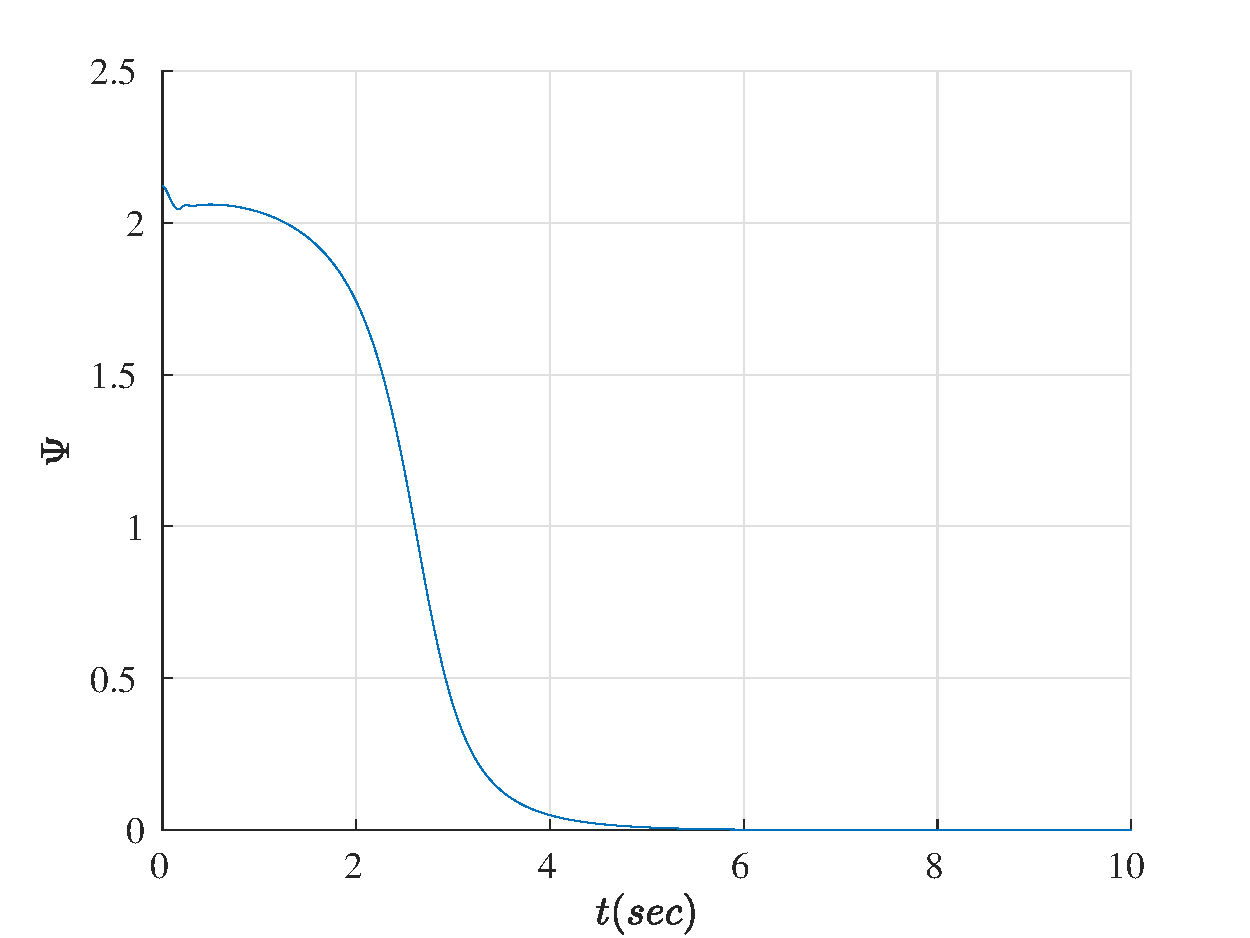
\includegraphics[width=0.5\columnwidth]{Psi_adapt} }~
-    \subfigure[Angle to constraints \label{fig:con_angles}]{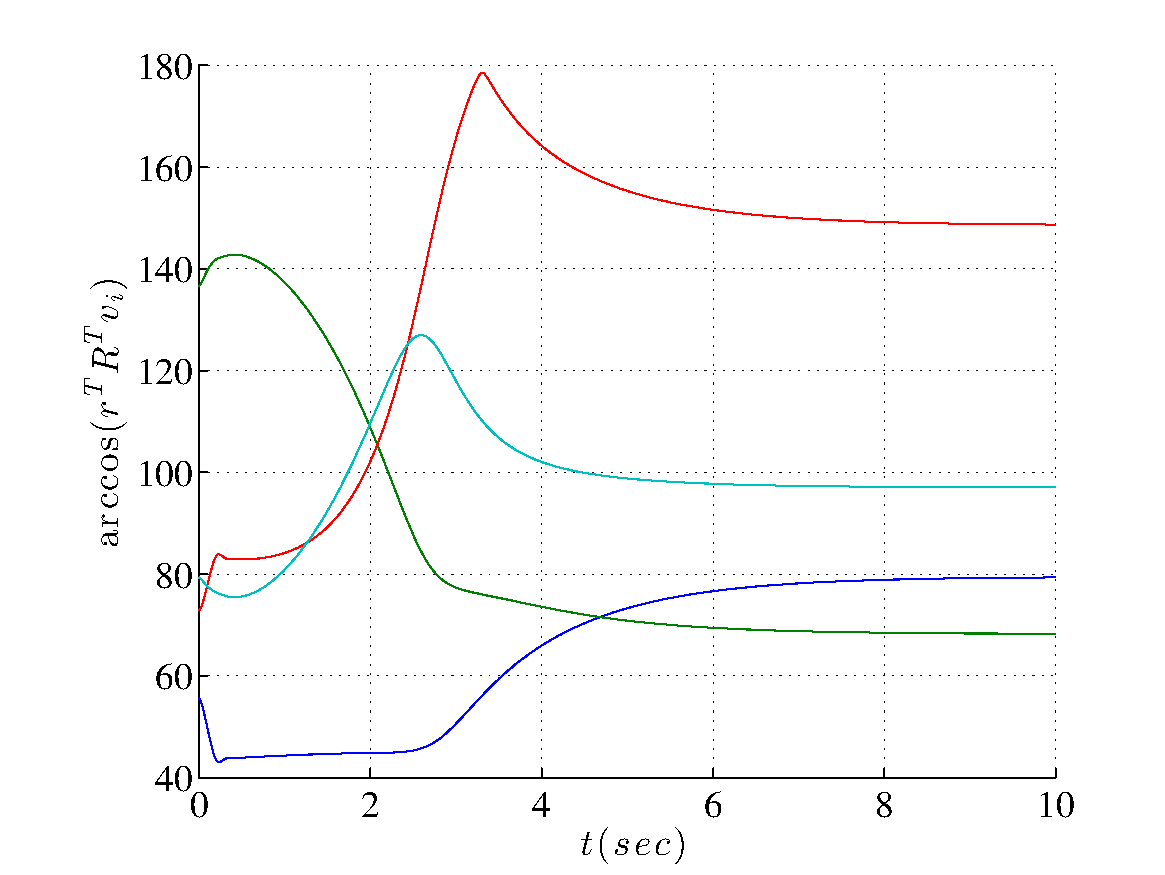
\includegraphics[width=0.5\columnwidth]{constraint_angles} }\\
-    \subfigure[Disturbance estimate \( \bar \Delta \)  \label{fig:delta_adapt} ]{\includegraphics[width=0.5\columnwidth]{delta_adapt}}~
-    \subfigure[Attitude trajectory \label{fig:cad_adapt}]{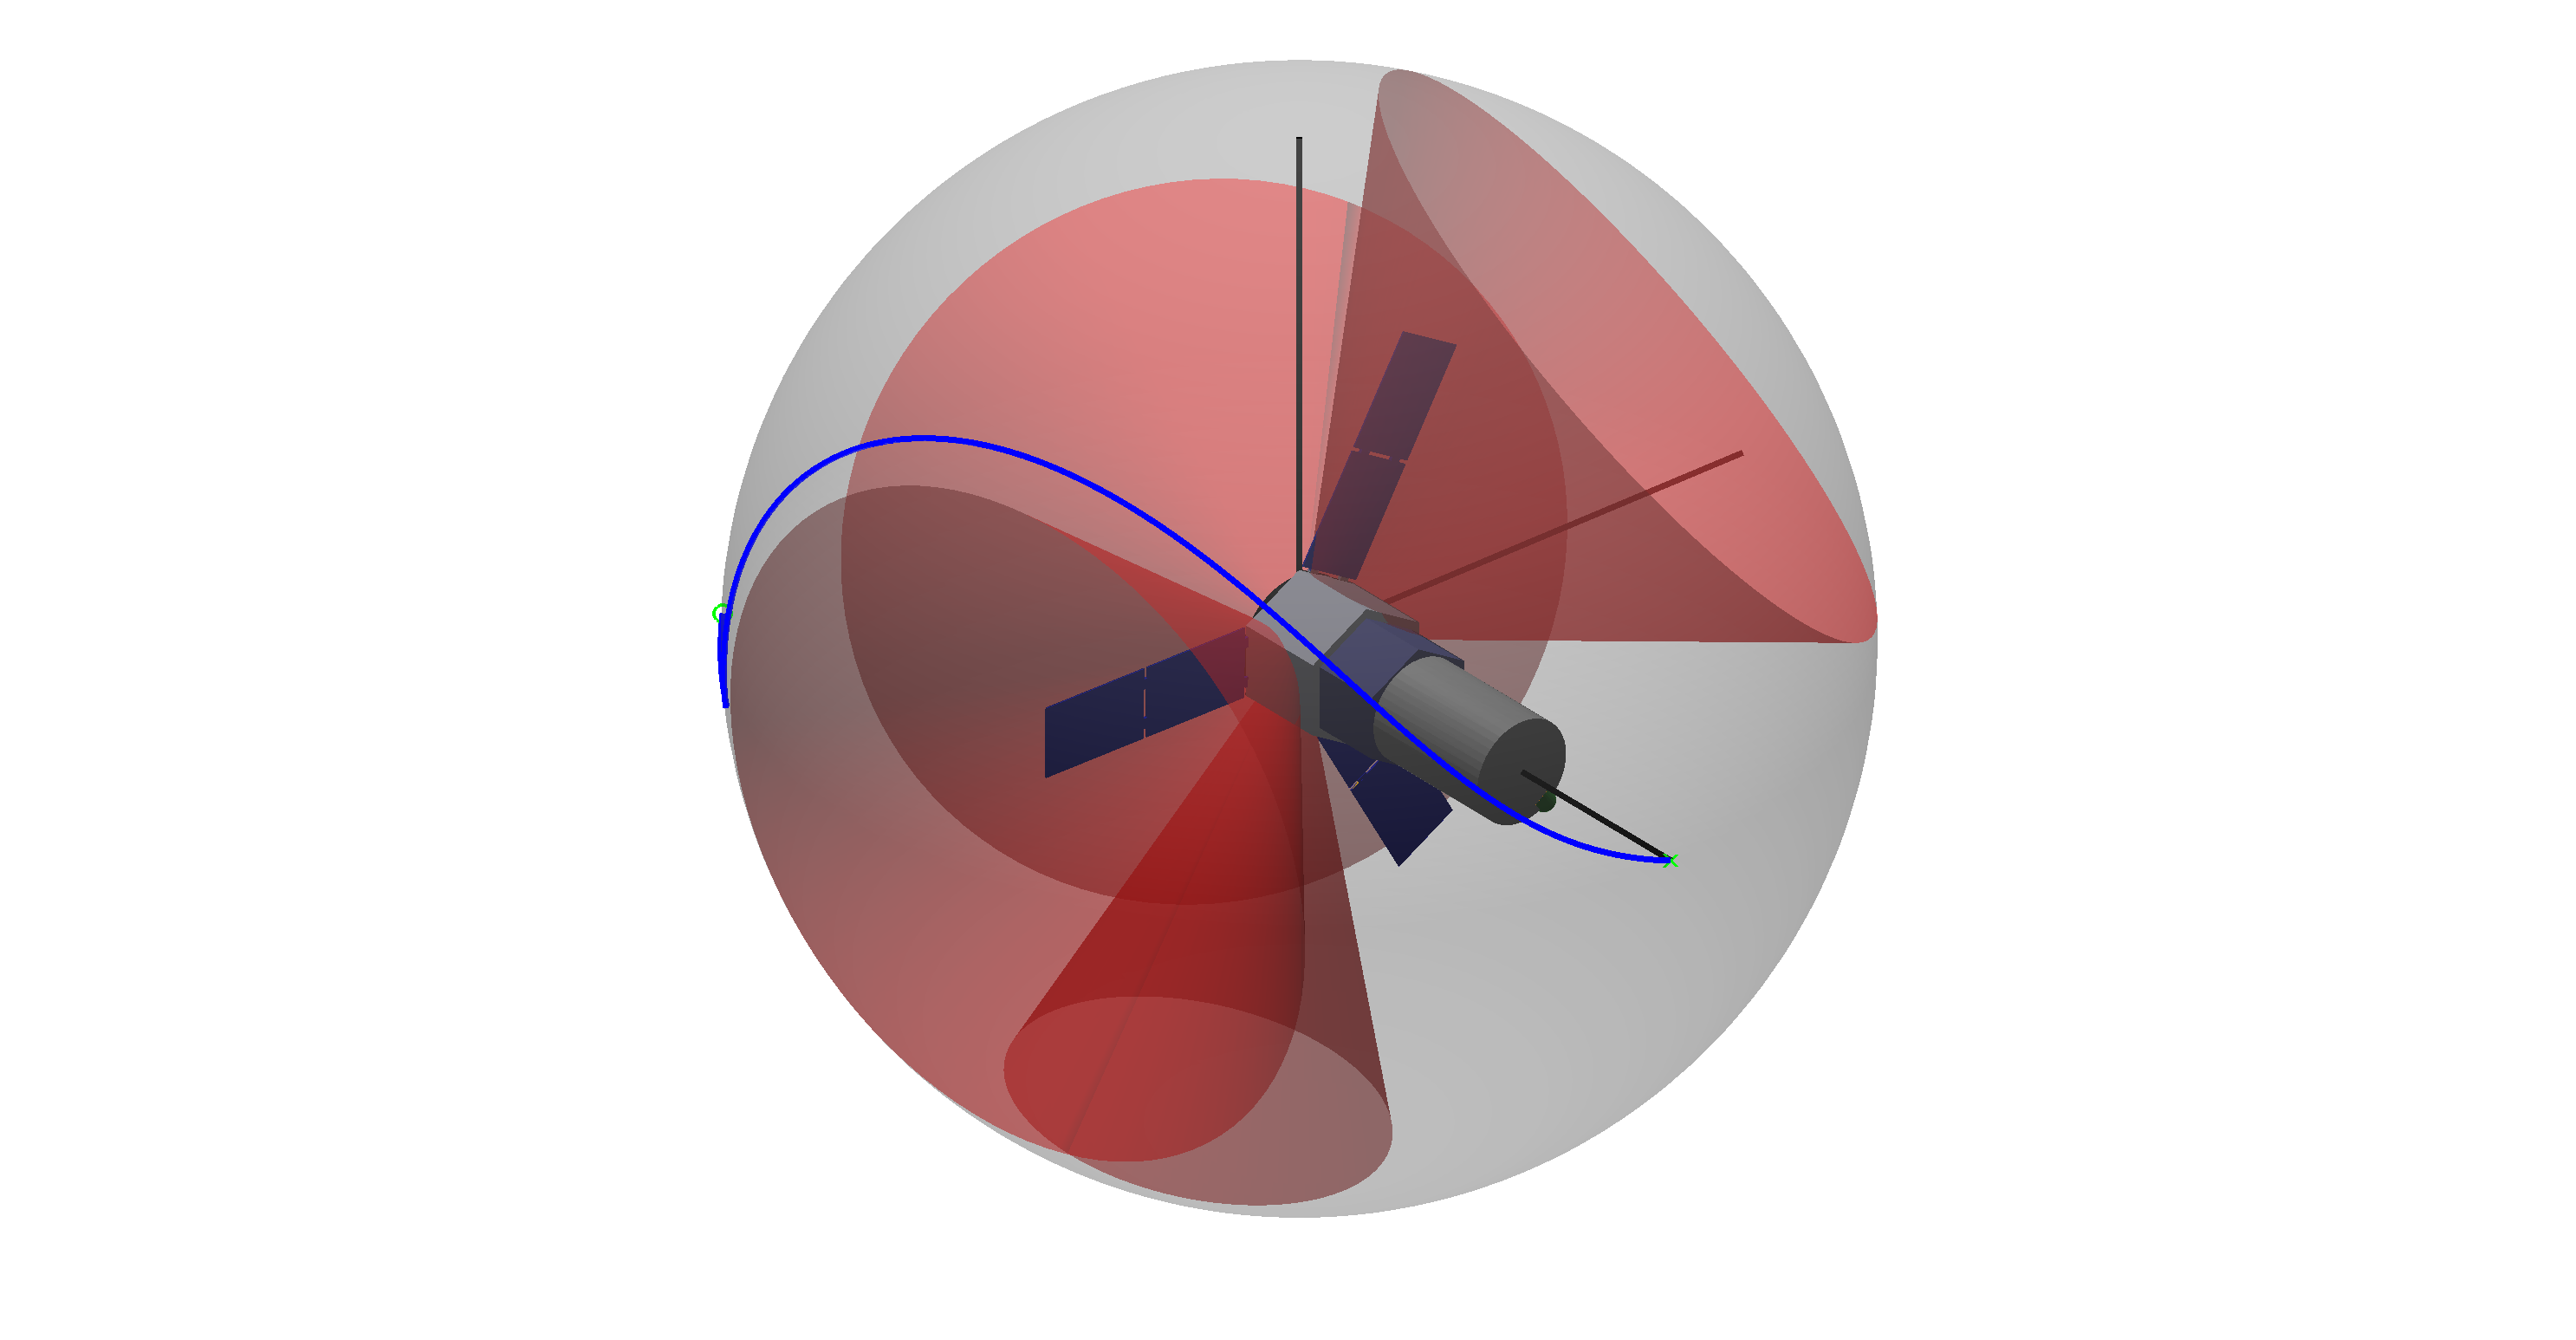
\includegraphics[trim=9cm 2.5cm 0 0,clip,width=0.645\columnwidth]{cad_adapt} }
-	\caption{Attitude stabilization with adaptive update law}
-	\label{fig:adapt} 
-\end{figure}
 
 Simulation results without the adaptive update law are shown in~\cref{fig:con}.
+\Cref{fig:eR_con} shows each component of the attitude error vector,~\cref{eqn:eR}, over the simulation time span.
+\Cref{fig:Psi_con} shows the  magnitude of the combined error function,~\cref{eqn:psi}.
 Without the update law, the system does not achieve zero steady state error. 
 \Cref{fig:Psi_con} shows that the configuration error function does not converge to zero and there exist steady state errors.
 In spite of the uncompensated disturbance, the system is able to avoid the constrained regions as shown in~\cref{fig:con_angles_con}.
-The angle to each of the constraints,  \( \arccos(r^T R^T v_i) \), is always greater than the specified angle, \( \theta_i \), in~\cref{tab:constraints}.
+The angle to each of the constraints, which is measured in degrees and given by \( \arccos(r^T R^T v_i) \), is always greater than the specified angle, \( \theta_i \), in~\Cref{tab:constraints}.
 
 \Cref{fig:adapt} shows the results with the addition of the adaptive update law.
+\Cref{fig:Psi_adapt,fig:con_angles} are equivalent to~\cref{fig:Psi_con,fig:con_angles_con} with the exception of the addition of the adaptive update law.
 The addition of the adaptive update law allows the system to converge to the desired attitude in the presence of constraints.
-The path of the body fixed sensor in the inertial frame, namely \( R r \), is illustrated in~\cref{fig:cad_adapt}.
-The initial attitude is represented with the green circle while the final attitude is marked with a green \(\times\).
+The path of the body fixed sensor in the inertial frame, namely \( R r \), is illustrated in~\cref{fig:cad_adapt} by the blue trajectory.
+The rendering of the spacecraft is presented in the desired, or final, orientation of the simulation.
 The inequality constraints from~\Cref{tab:constraints} are depicted as red cones, where the cone half angle is \( \theta \).
 The control system is able to asymptotically converge to zero attitude error.
-\Cref{fig:con_angles} shows that the angle \( \arccos(r^T R^T v_i) \) between the body fixed sensor and each constraint is satisfied for the entire maneuver.
+\Cref{fig:con_angles} shows that the angle, \( \arccos(r^T R^T v_i) \) and measured in degrees, between the body fixed sensor and each constraint is satisfied for the entire maneuver.
 In addition, the estimate of the disturbance converges to the the true value as shown in~\cref{fig:delta_adapt}.
 
 Both control system are able to automatically avoid the constrained regions. 
@@ -487,8 +514,107 @@ In spite of this challenging configuration space, the proposed control system of
 These closed-loop feedback results are computed in real time and offer a significant advantage over typical open-loop planning methods.
 These results show that the proposed geometric adaptive approach is critical to attitude stabilization in the presence of state constraints and disturbances.
 
-\section{Experiment on Hexrotor UAV}
+\subsection{Attitude Parameterizations}\label{ssec:attitude_parameterization}
+\end{multicols}
+\begin{figure} 
+  \centering 
+    \subfigure[Configuration error \( \Psi \)\label{fig:Psi_adapt}]{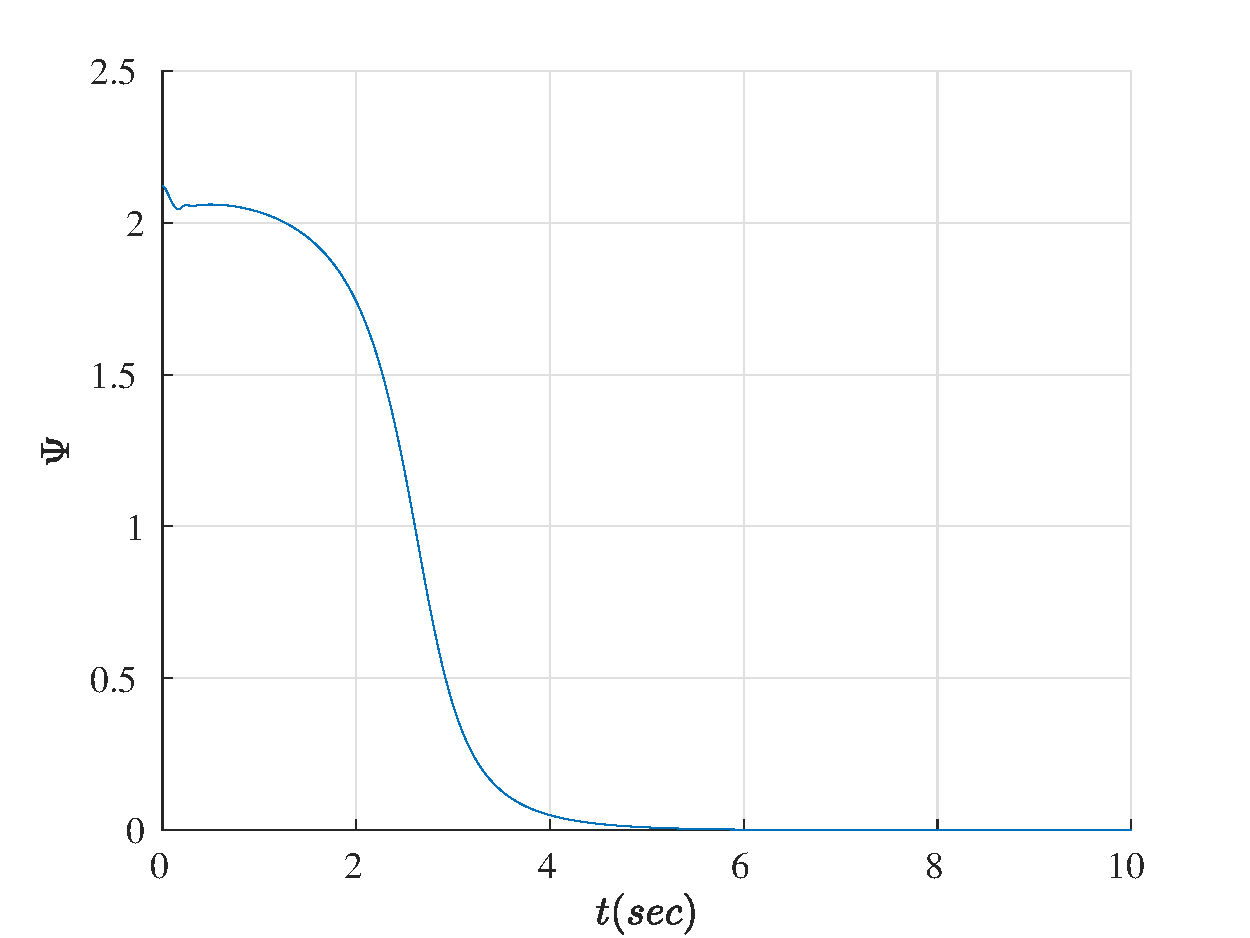
\includegraphics[width=0.4\columnwidth]{Psi_adapt} }~
+    \subfigure[Angle to each constraint \label{fig:con_angles}]{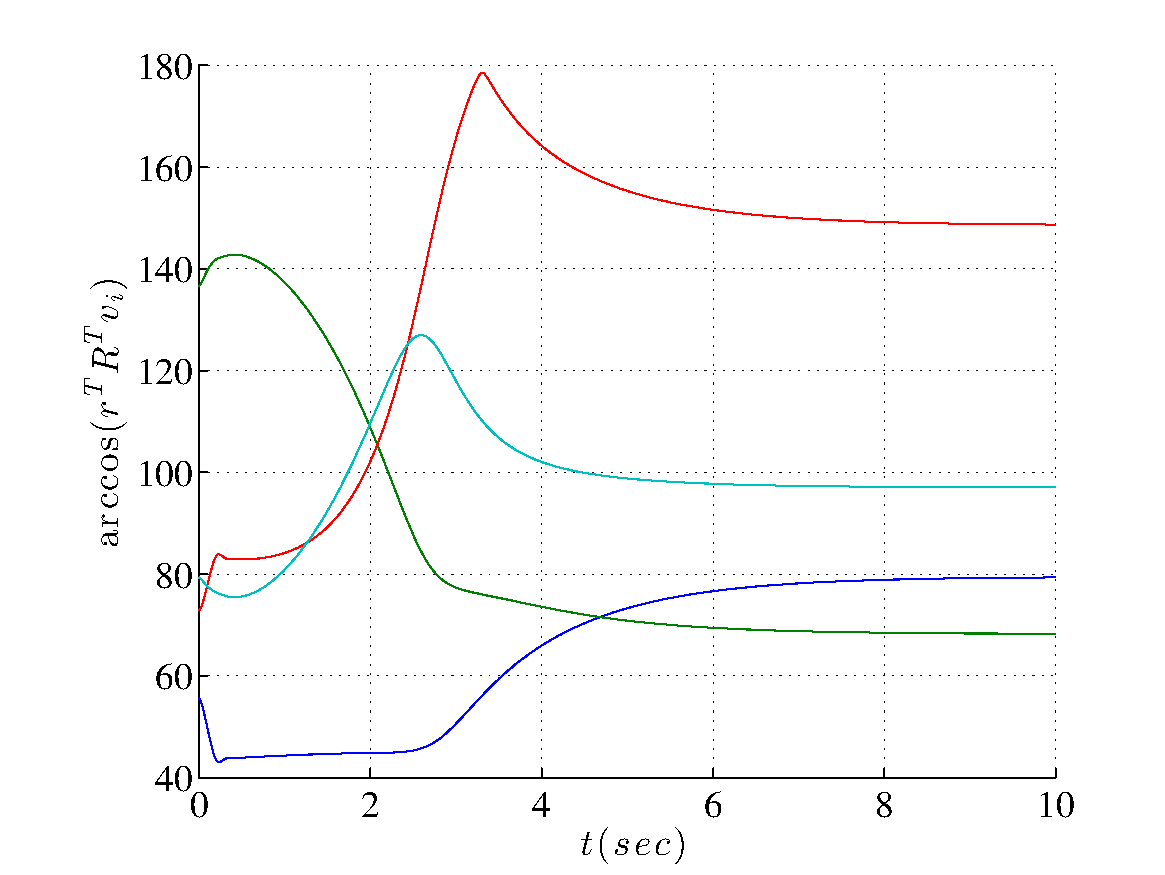
\includegraphics[width=0.4\columnwidth]{constraint_angles} }\\
+    \subfigure[Disturbance estimate \( \bar \Delta \) components \label{fig:delta_adapt} ]{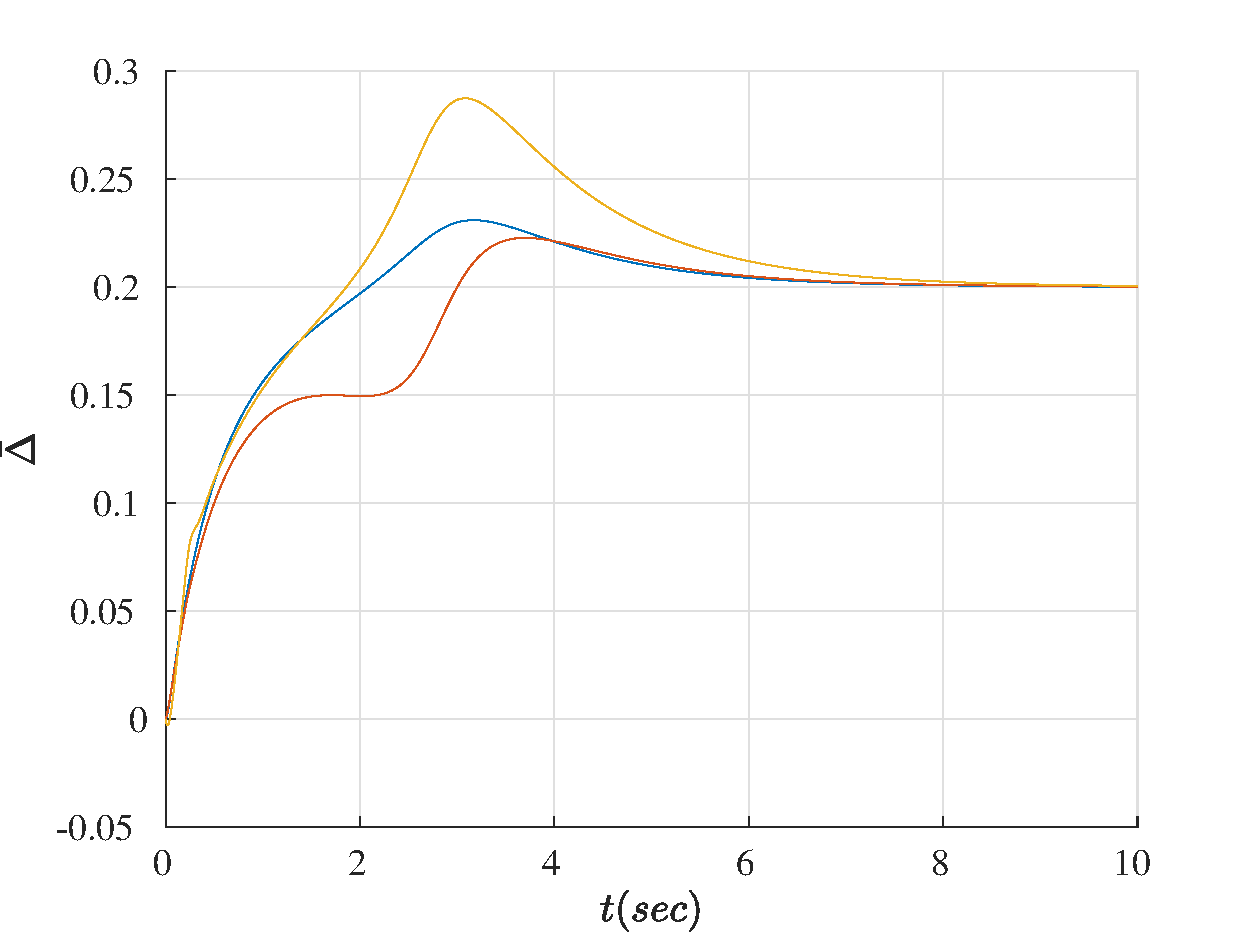
\includegraphics[width=0.4\columnwidth]{Delta_adapt}}~
+    \subfigure[Attitude trajectory \label{fig:cad_adapt}]{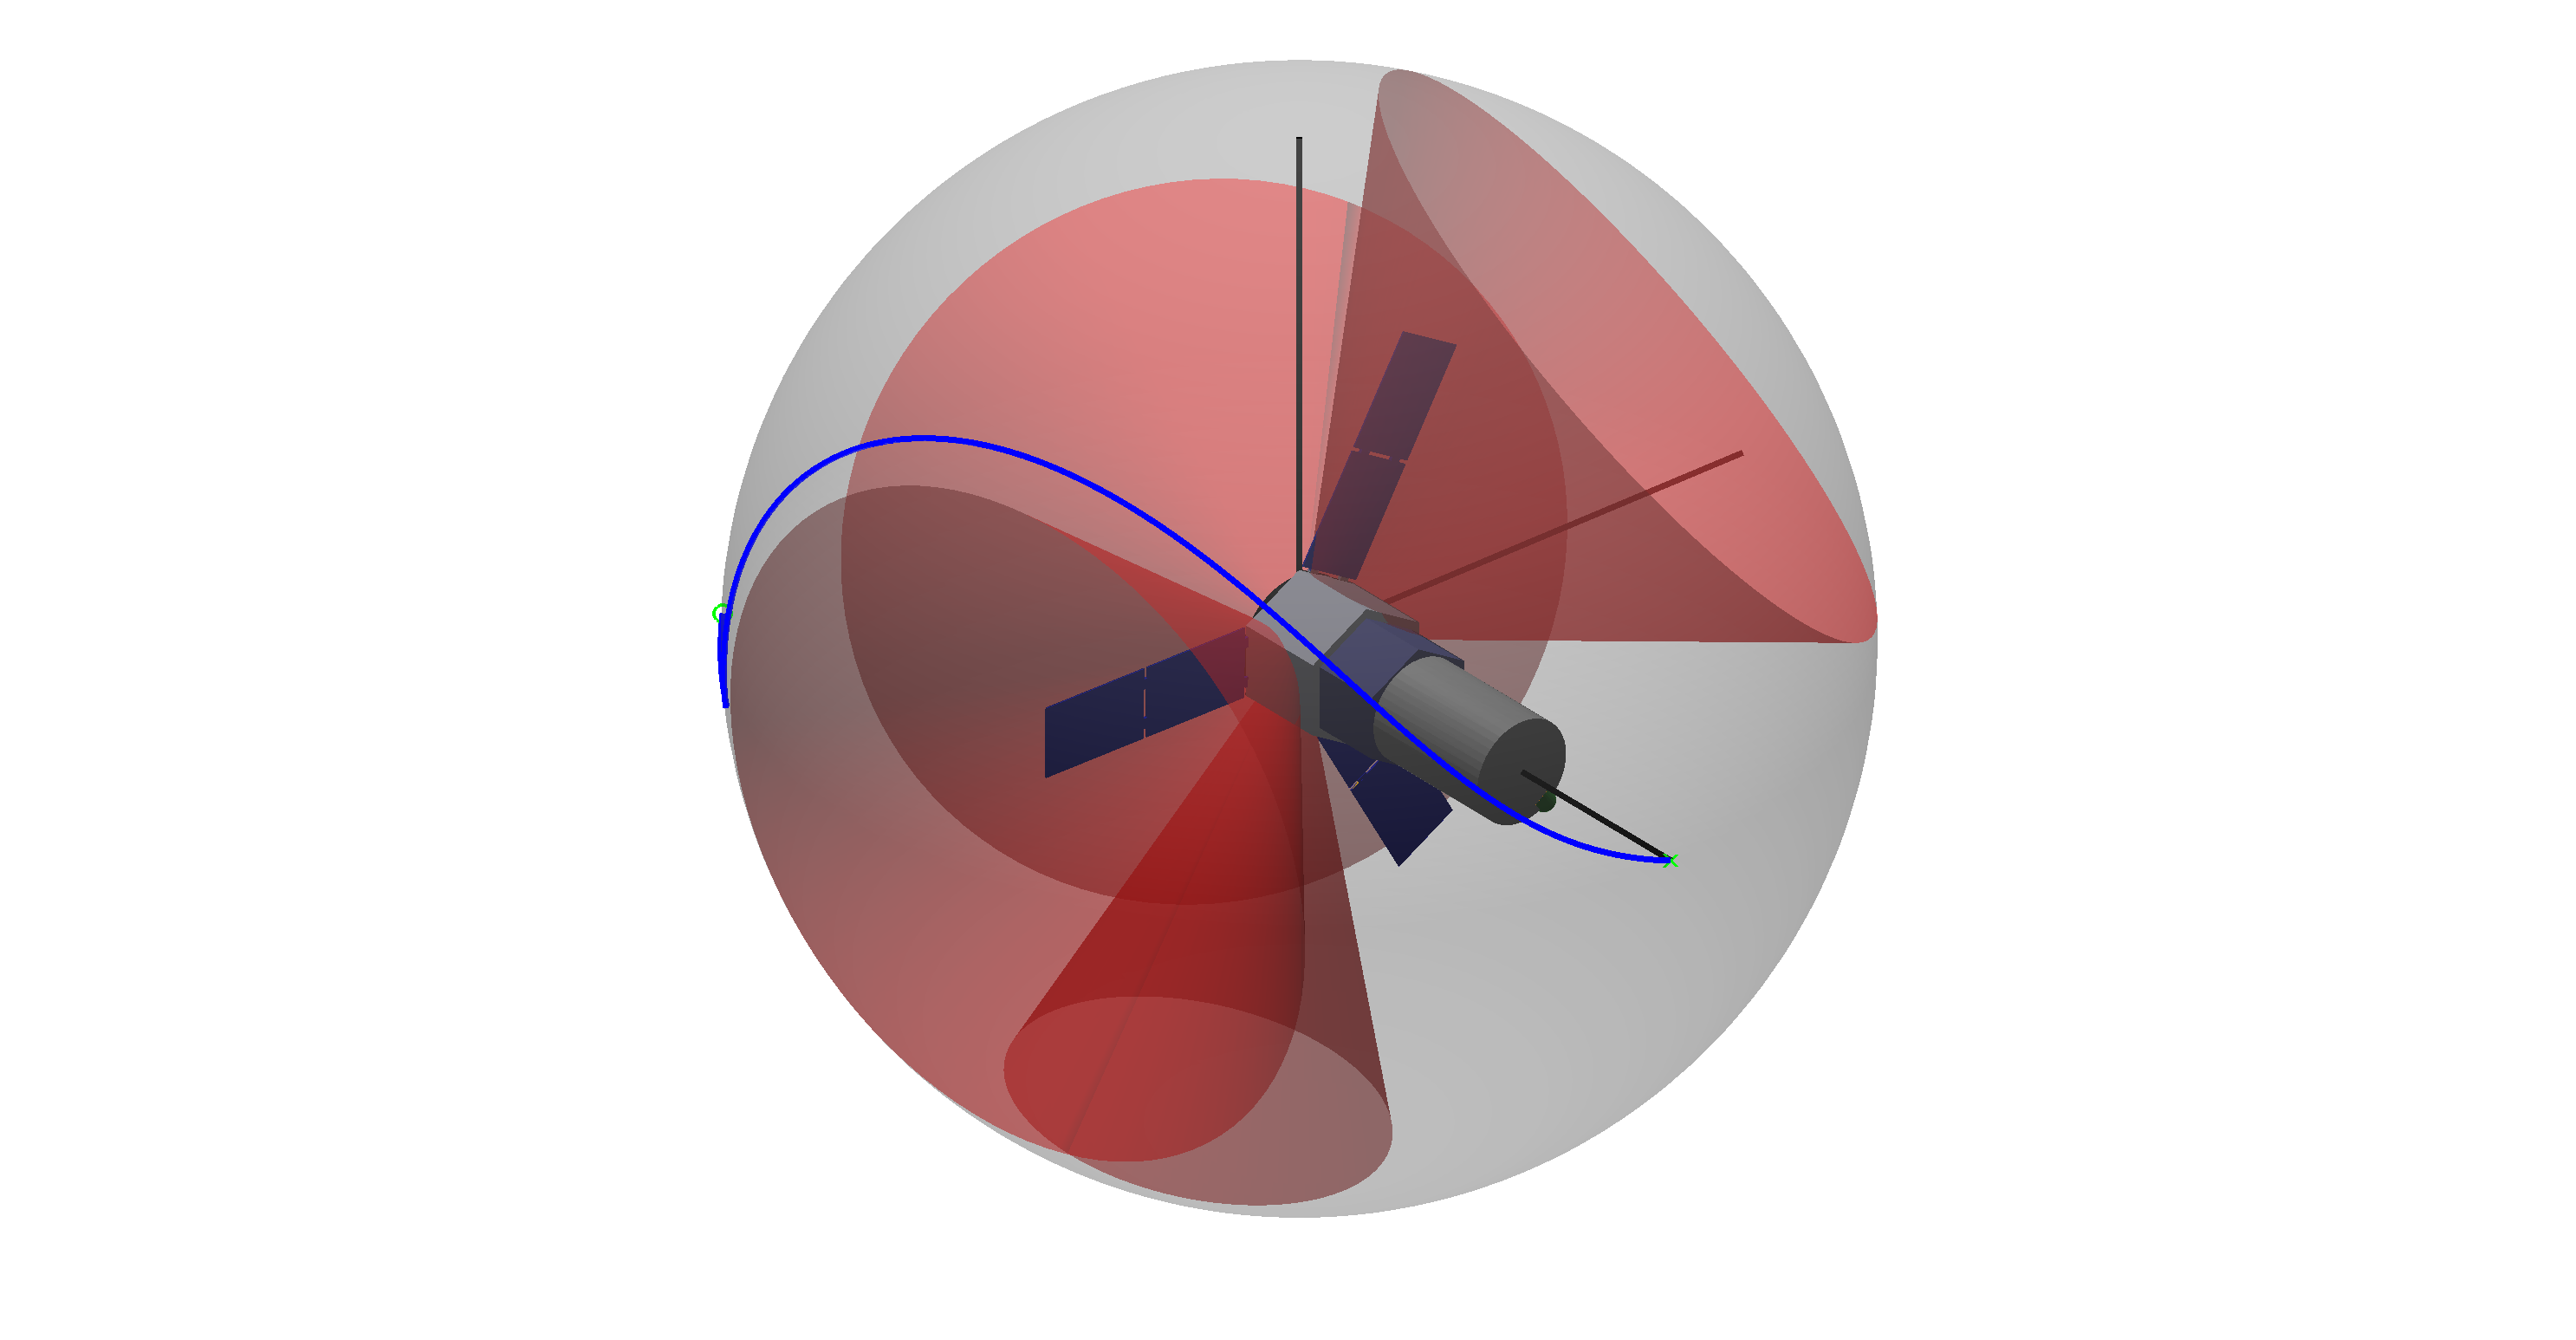
\includegraphics[trim={10cm 0 10cm 0},clip,width=0.4\columnwidth]{cad_adapt} }
+  \caption{Attitude stabilization with adaptive update law}
+  \label{fig:adapt} 
+\end{figure}
+\begin{multicols}{2}
+% Discuss the benefits of using this geometric representation as compared to Euler angles or quaternions
+Attitude parameterizations, such as Euler angles and Quaternions, are frequently used in the aerospace and astrodynamics communities~\cite{vallado2007}.
+For example, Euler angle sequences are frequently used to describe the transformation between a variety of reference frames used to describe the position and orientation of the orbit of Earth satellites~\cite{vallado2007}.
+In addition, quaternions were used during the operation of Skylab and the NASA Space Shuttle~\cite{hughes2004}.
+However, the choice of attitude parameterization plays a critical role in control design and the resulting motion of the system.
+
+% singularities and the problems involved with using Euler angles
+Euler angle sequences are a minimum, three-parameter set of angles which describe the transformation between two reference frames.
+Using Euler angles, we can represent any general rotation as a sequence of three intermediate rotations~\cite{shuster1993}.
+By convention, there are \num{24} possible Euler angle sequences for any given rotation.
+In addition, Euler angles are a minimum representation, as only three angles, and the associated sequence, are required to describe the three angular degrees of freedom of the rigid body.
+However, there is great ambiguity in the representation of the attitude as there are many equivalent Euler angle sequences for a given attitude of the system.
+Therefore, great care must be taken in the control system design to ensure that a consistent sequence is used. 
+Furthermore, it has been shown that no minimal attitude representation can describe orientations both globally and without singularities~\cite{hughes2004,bhat2000}.
+These singularities can cause significant difficulties during control design and hardware implementation.
+
+To demonstrate the effect of the kinematic singularities inherent with Euler angles we will represent the attitude of the body fixed reference frame, \( \vecbf{b}_i \), with respect to the inertial frame, \( \vecbf{e}_i\), in terms of the \( 3-1-3\) Euler angle sequence.
+More explicitly, this corresponds to the rotation sequence \( \theta_1 \vecbf{b}_3 , \theta_2 \vecbf{b}_1, \theta_3 \vecbf{b}_3 \).
+The rotation matrix, \( R(\theta_1, \theta_2, \theta_3) \), corresponding to this sequence is 
+\begin{align}\label{eq:euler313}
+    \begin{bmatrix}
+        -s_1 c_2 s_3 + c_3 c_1 & -s_1 c_2 c_3 - s_3 c_1 & s_1s_2 \\
+        c_1 c_2 s_3 + c_3 s_1 & c_1 c_2 c_3 - s_3 s_1 & - c_1 s_2 \\
+        s_2 s_3 & s_2 c_3 & c_2
+    \end{bmatrix} ,
+\end{align}
+where \( s_i, c_i \) represent \( \sin \theta_i, \cos \theta_i \) for \( i = \braces{1,2,3}\).
+Using this representation, the kinematic differential equations for the associated Euler angles are given as
+\begin{align}\label{eq:euler313_diff}
+    \begin{bmatrix}
+        \dot{\theta}_1 \\ \dot{\theta}_2 \\ \dot{\theta}_3 
+    \end{bmatrix}
+    =
+    \begin{bmatrix}
+        \slfrac{\parenth{\Omega_1 s_3 + \Omega_2 c_3}}{s_2} \\
+        \Omega_1 c_3 - \Omega_2 s_3 \\
+        -\slfrac{\parenth{\Omega_1 s_3 + \omega_2 c_3}c_2}{s_2} + \Omega_3
+    \end{bmatrix} .
+\end{align}
+From~\cref{eq:euler313_diff}, it is immediately clear that a singularity exists when \( \sin \theta_2 = 0 \) or equivalently, \( \theta_2 = 0, \pm \pi \). 
+In the vicinity of the singularity, the angular velocities of the Euler angles will tend to approach \( \pm \infty \) and the angular velocities will experience instantaneous sign changes.
+Furthermore, all Euler angle sequences will exhibit a similar singularity at either \( \theta_2 = 0, \pm \pi \) or \( \theta_2 = \pm \frac{\pi}{2}, \pm \frac{3\pi}{2} \).
+Therefore simply switching the sequence does not alleviate the issue, but rather only moves the singularity.
+As a result, Euler angles are not appropriate for systems which experience large angular rotations, such as those demonstrated in~\cref{fig:adapt}, or control systems which rely on the angular velocities \( \theta_i \).
+% discuss the unwinding phenomenon with quaternions
+
+\end{multicols}
+\begin{figure}[h]
+    \centering 
+    \subfigure[{Configuration error \( \Psi \)} \label{fig:Psi_tv} ]{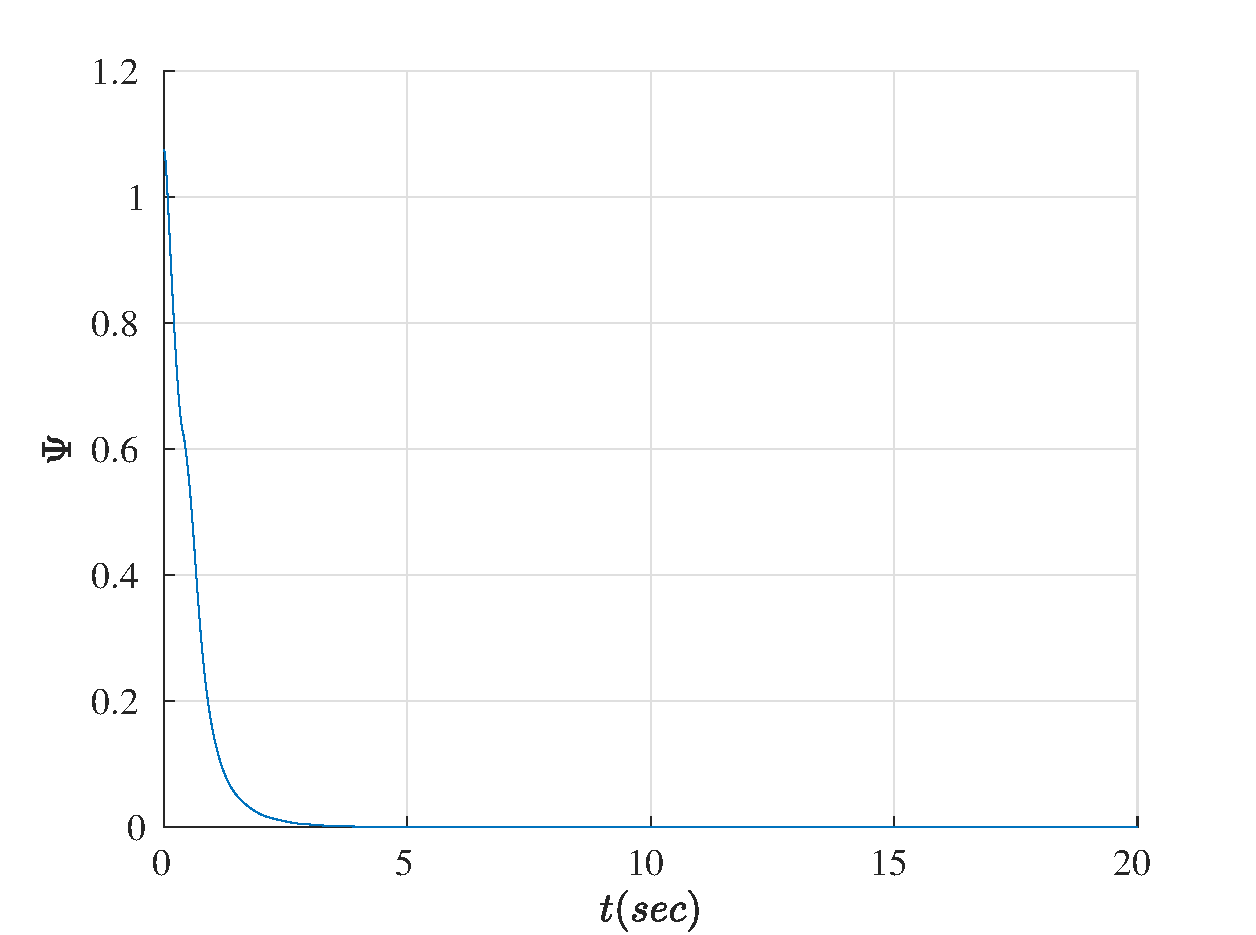
\includegraphics[width=0.3\columnwidth]{Psi_tv} }~
+    \subfigure[{Angle to constraint } \label{fig:con_angle_tv}]{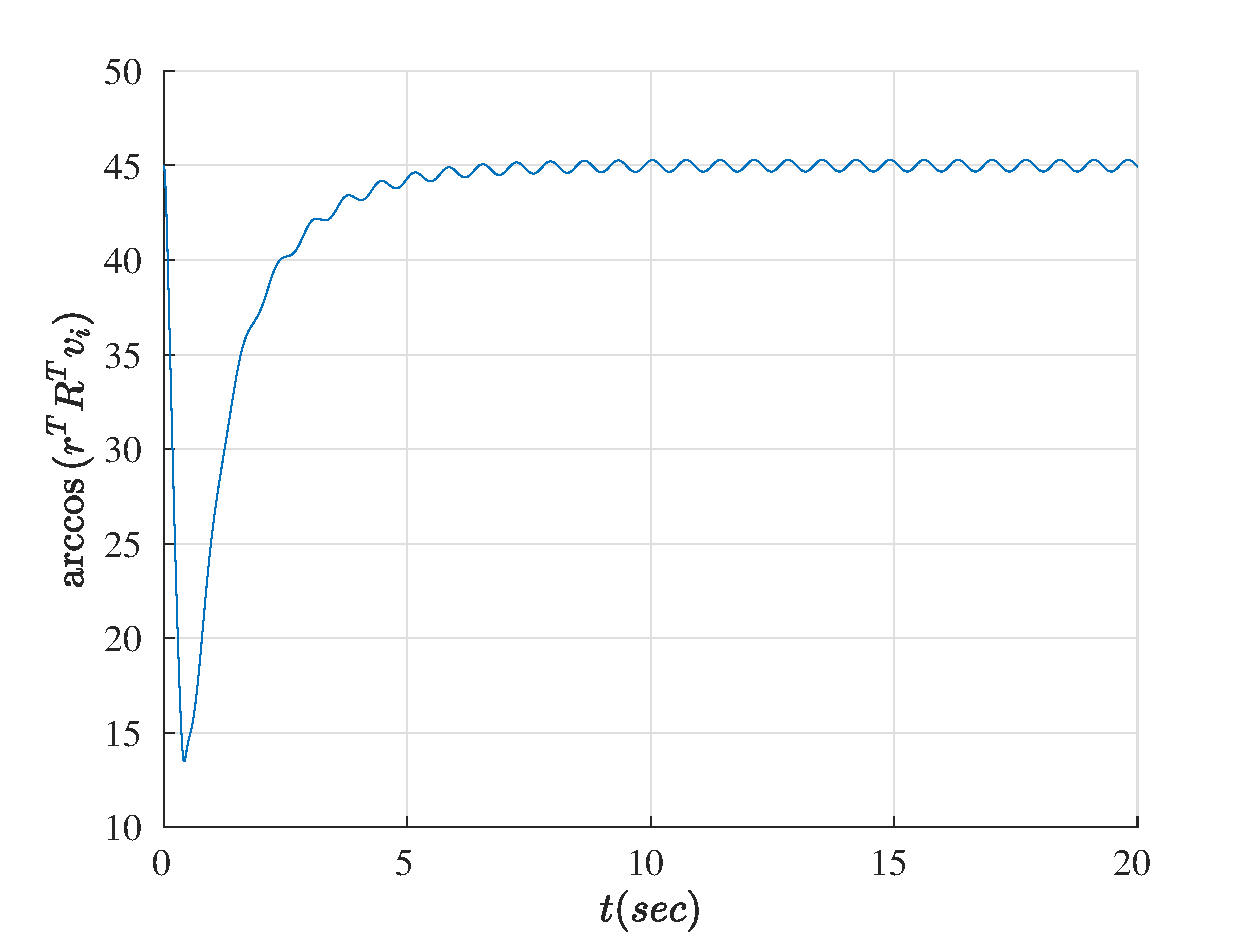
\includegraphics[width=0.3\columnwidth]{figures/constraint_angle_tv.pdf} }~
+    \subfigure[{Disturbance estimate \(\bar\Delta\) components} \label{fig:Delta_tv}]{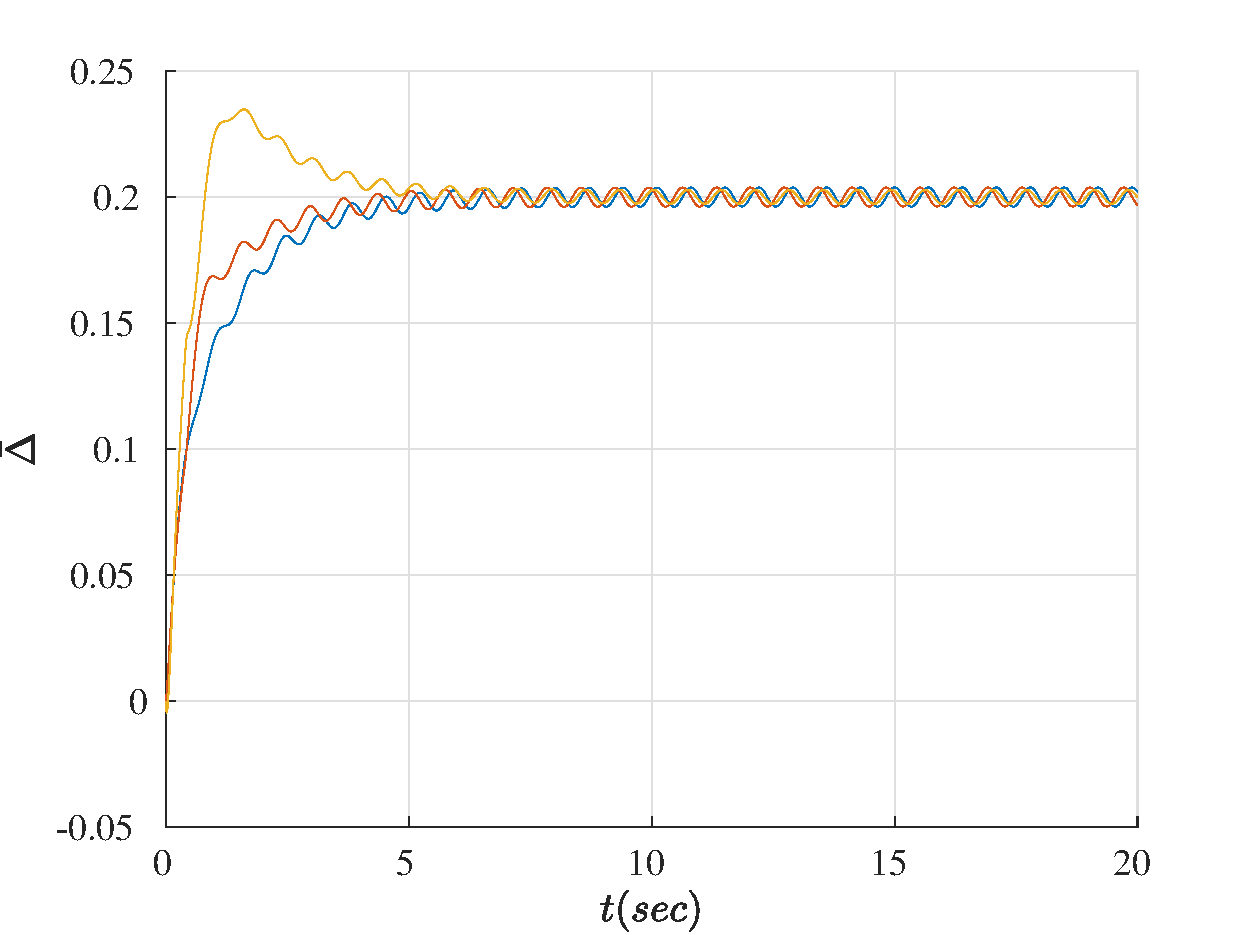
\includegraphics[width=0.3\columnwidth]{figures/delta_tv} }
+    \caption{Time-varying external disturbance simulation}
+    \label{fig:tv} 
+\end{figure}
+\begin{multicols}{2}
+\subsection{Time-varying Disturbance}\label{ssec:time_varying}
+
+The form of the uncertainty, given in~\cref{eqn:Wdot}, is commonly used in the adaptive control literature~\cite{LeeITCST13,ioannou2012}. 
+A wide variety of realistic disturbances, such as gravitational gradients or malfunctioning thrusters for spacecraft scenarios, are accurately represented via this model. 
+In addition, it is possible to represent the uncertainty of a time-varying inertia matrix as an equivalent external disturbance. 
+For example, Euler's law gives the relationship for the rate of change of angular momentum as
+\begin{align*}
+    M_{ext} = \dot{\vecbf{H}} = \dot{J} \vecbf{\Omega} + J \dot{\vecbf{\Omega}} .
+\end{align*}
+Using this, we can see that an instantaneous change in \( J \) is proportional to an external moment.
+Finally, it has been shown that this adaptive control formulation is able to handle time-varying disturbances under some mild assumptions~\cite{ioannou2012}. 
 
+We demonstrate the ability to handle an uncertain time-varying disturbance via numerical example.
+The system is identical to the one presented in~\cref{sec:numerical_simulation}, however we modify the external disturbance. 
+The external disturbance is the superposition of constant and time-varying terms as
+\begin{align*}
+    \Delta = \begin{bmatrix} 0.2 \\ 0.2 \\0.2 \end{bmatrix} + 0.02 \begin{bmatrix} \sin 9 t \\ \cos 9 t \\ \frac{1}{2} \parenth{\sin 9t + \cos 9t}\end{bmatrix} \si{\newton\meter}.
+\end{align*}
+We define a constraint in the inertial frame as \( v = [\frac{1}{\sqrt{2}}, \frac{1}{\sqrt{2}}, 0]^T \) with \( \theta = \ang{12} \).
+The initial state is defined as \(R(0) = \exp( \frac{\pi}{2} \hat{e}_3) \), while the desired state is \(R_d =I \).
+The goal is to rotate the vehicle about the \( e_3 \) axis while avoiding the obstacle and compensating for the time-varying disturbance. 
+
+\Cref{fig:tv} demonstrates the ability for the adaptive controller, which is presented in~\Cref{prop:adaptive_control}, to handle time-varying disturbances.
+\Cref{fig:Psi_tv} shows the non-dimensional value of the configuration error function and demonstrates that the adaptive controller is able to stabilize the system to the desired attitude configuration.
+In addition,~\cref{fig:con_angle_tv} shows that the constraint is never violated as the angle between the body-fixed sensor \( r \) and the constraint \( v \) is greater than \SI{12}{\degree} over the entire attitude maneuver.
+We can see in~\cref{fig:Delta_tv} that that estimate \(\bar \Delta \) for each of the components accurately tracks the true disturbance after approximately~\SI{5}{\second}.
+
+\section{Experiment on Hexrotor UAV}\label{sec:experiment}
+\begin{figure}[H]
+    \centering
+    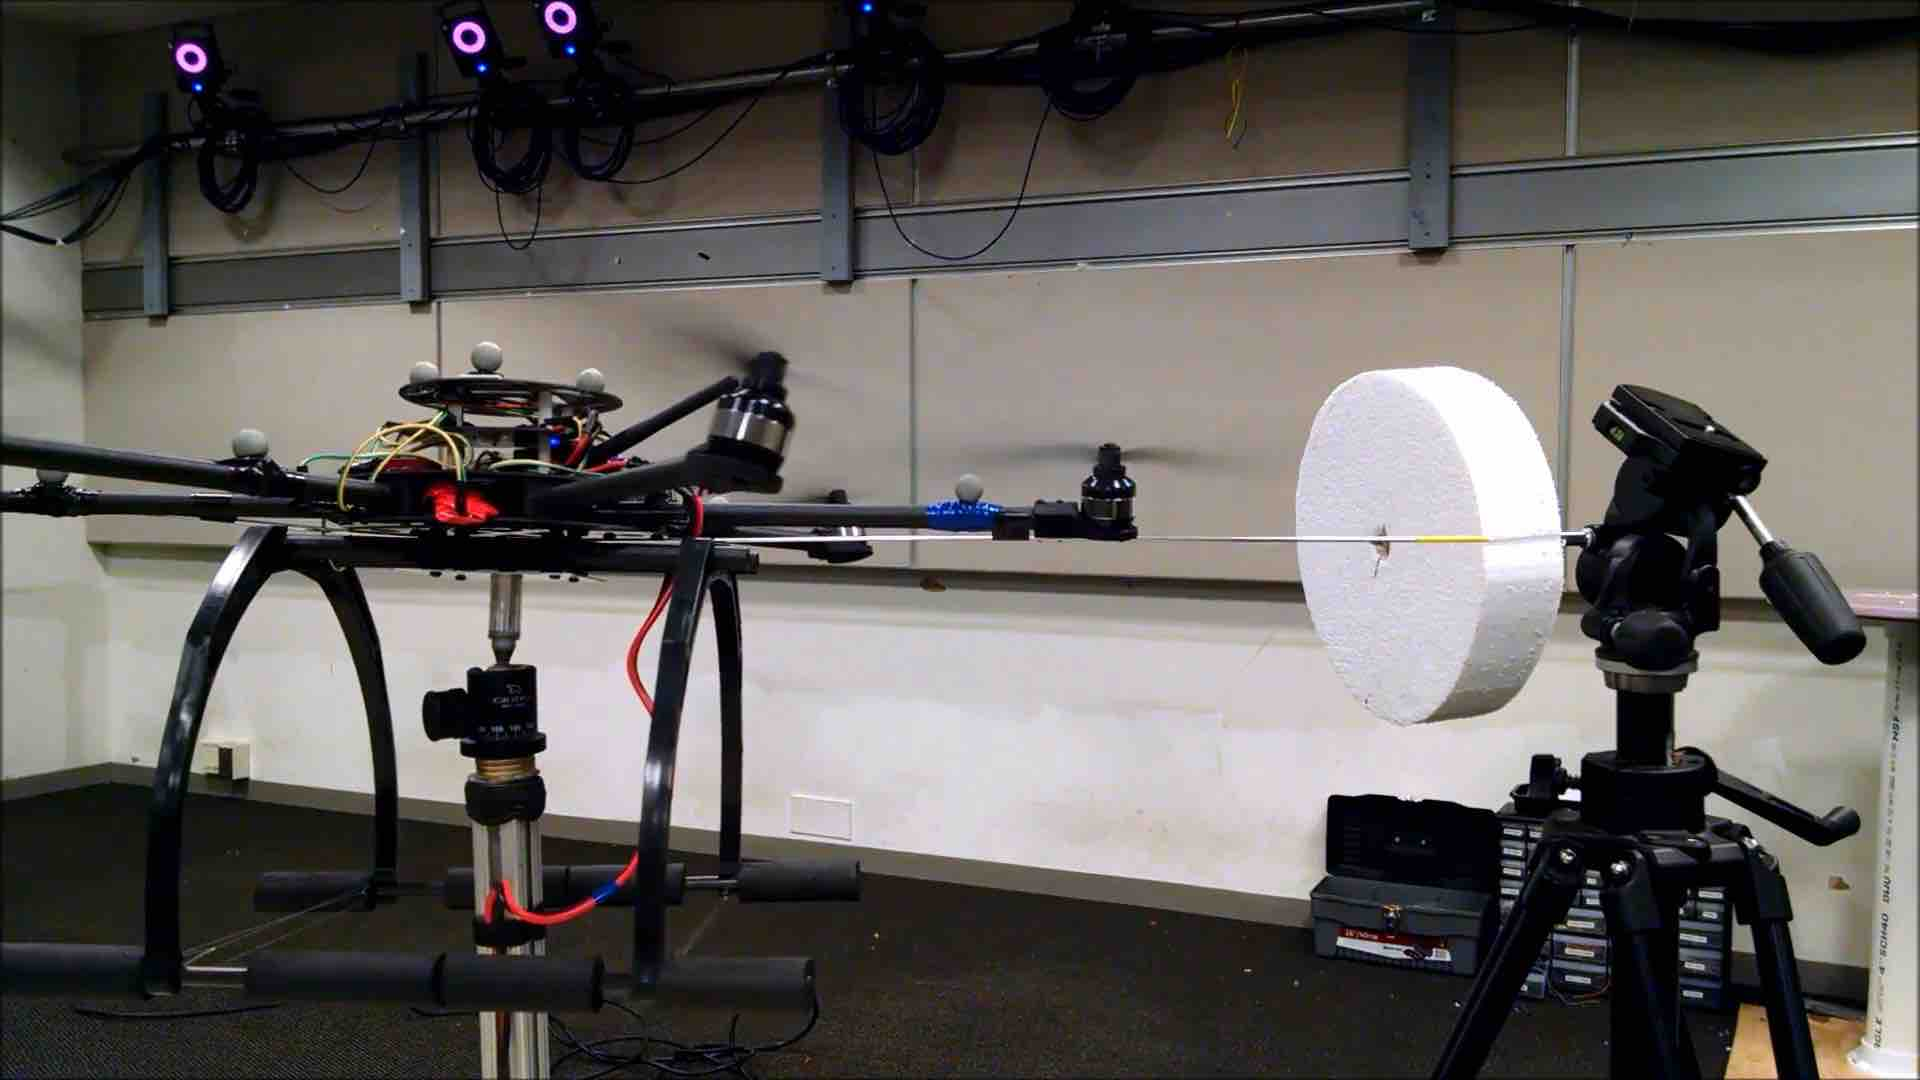
\includegraphics[width = 0.75\columnwidth]{hexrotor}
+    \caption{Attitude control testbed~\label{fig:hexrotor}}
+\end{figure}
 A hexrotor unmanned aerial vehicle (UAV), as seen in~\cref{fig:hexrotor}, has been developed at the Flight Dynamics and Controls Laboratory (FDCL) at the George Washington University~\cite{kaufman2014}.
 The UAV is composed of three pairs of counter-rotating propellers. 
 Typical UAVs are composed of four or more co-planar propellers.
@@ -497,13 +623,12 @@ For example, quadrotor UAVs are unable to translate laterally without first cond
 Conversely, the propeller pairs of the hexrotor are angled relative to one another to allow for a fully actuated rigid body.
 This allows the hexrotor to impart a force in any direction and a moment about any axis. 
 
-\begin{figure}[H]
-    \centering
-    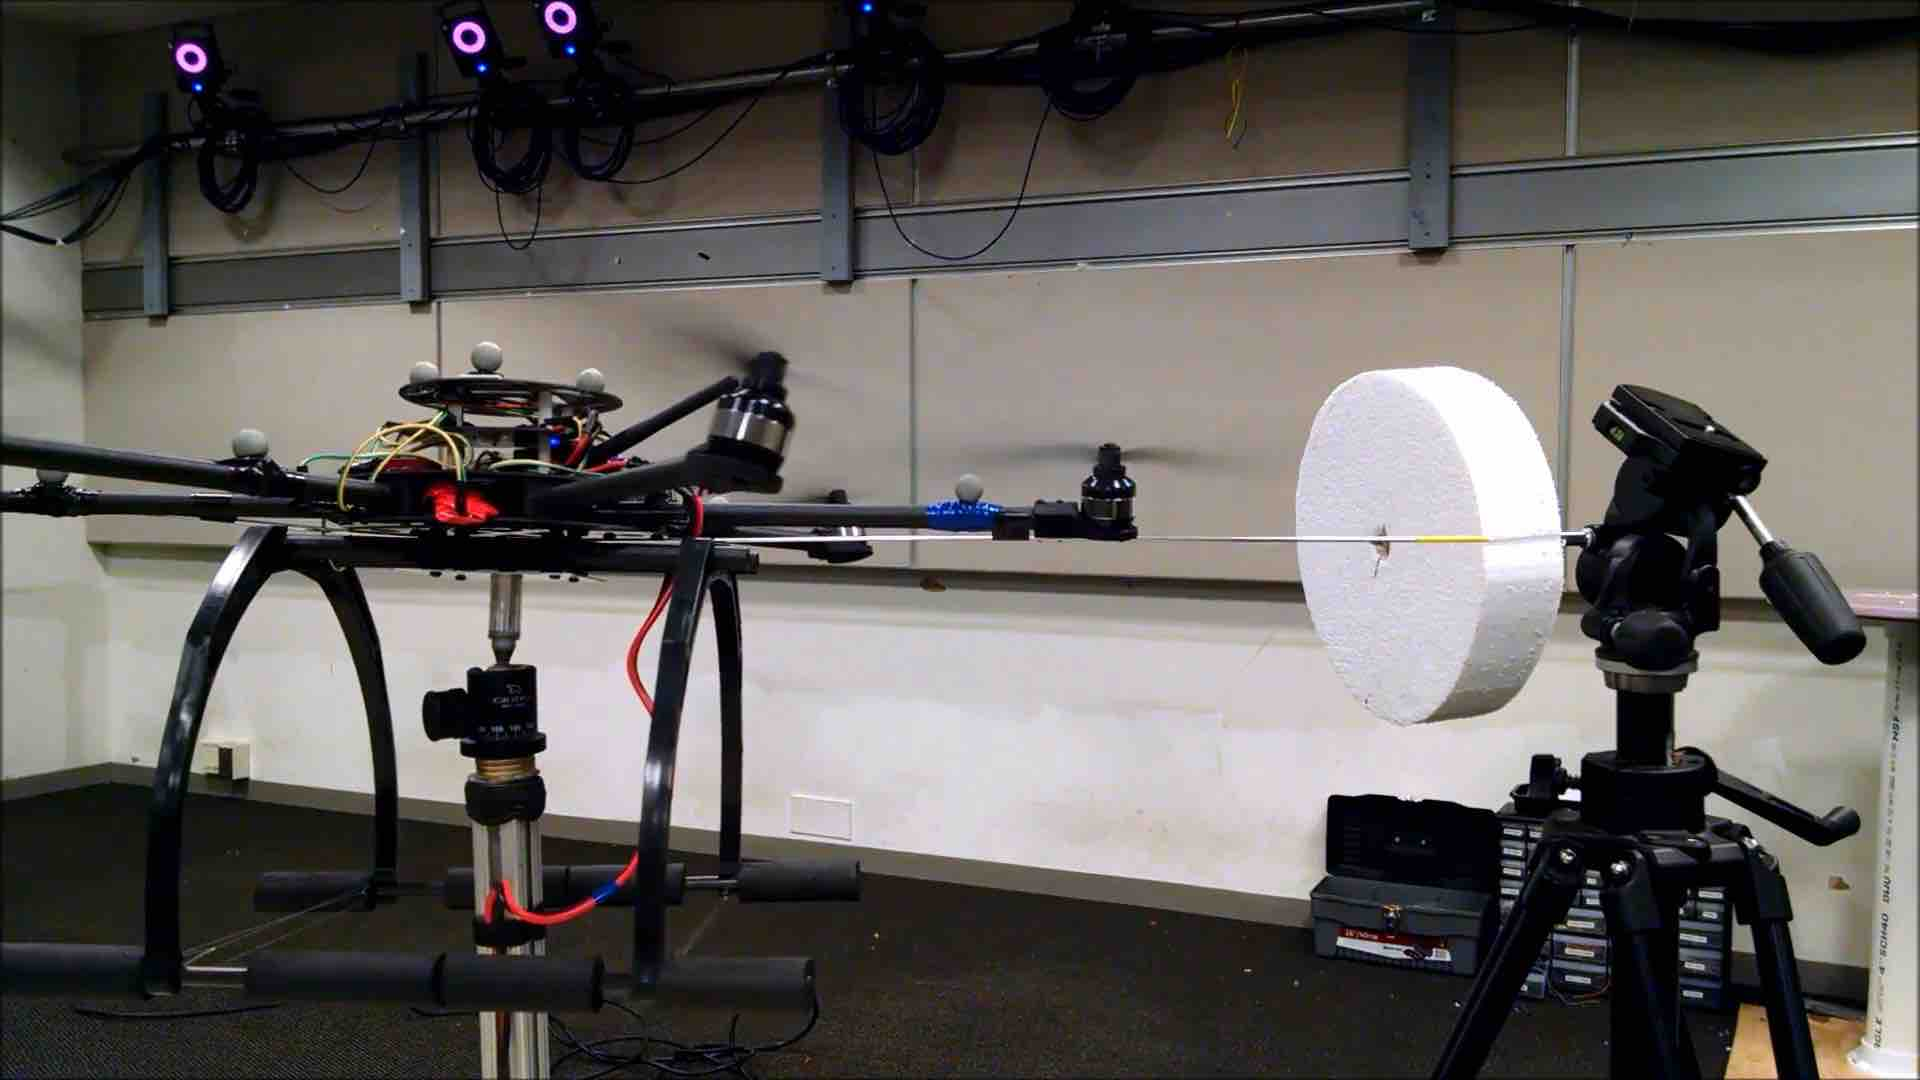
\includegraphics[width = 0.75\columnwidth]{hexrotor}
-    \caption{Attitude control testbed~\label{fig:hexrotor}}
-\end{figure}
-Attitude information is measured by an onboard IMU and a Vicon motion capture system in the test area.
-The control input is computed onboard the hexrotor using data transmitted via WiFi in a client/server model.
+Attitude information is measured by a combination of both on and off board sensor systems.
+The VectorNav VN-100 is a rugged, miniature high-performance inertial measurement unit which provides high frequency angular velocity measurements.
+A Vicon motion capture system is installed within the test environment and used to provide high accuracy attitude measurements. 
+A series of reflective markers are placed on the hexrotor and their relative position is captured by a series of infrared optical cameras. 
+Assuming a fixed rigid body, the Vicon system is able to derive the attitude of the hexrotor and transmit this data to the processor onboard the hexrotor.
+The control input is computed on-board, using the full state measurement, and implemented at approximately \SI{100}{\hertz}.
 In order to constrain the motion, allowing us to test only the attitude dynamics, we attach the hexrotor to a spherical joint.
 Since, the center of rotation is below the center of gravity of the hexrotor there is a destabilizing gravitational moment.
 The resulting attitude dynamics are similar to an inverted pendulum model.
@@ -513,27 +638,35 @@ A sensor pointing direction is defined in the body-fixed frame of the hexrotor a
 We define an obstacle in the inertial frame as \( v = [\frac{1}{\sqrt{2}}, \frac{1}{\sqrt{2}}, 0]^T \) with \( \theta = \ang{12} \).
 An initial state is defined as \(R(0) = \exp( \frac{\pi}{2} \hat{e}_3) \), while the desired state is \(R_d =I \).
 This results in the UAV performing a \ang{90} yaw rotation about the vertical axis of the spherical joint and the constrained region is on the shortest path connecting $R_0$ and $R_d$. 
-The attitude control system is identical to the one presented in~\Cref{prop:adaptive_control} with the exception of a gravity moment term and the following parameters: \(k_R = 0.4, k_\Omega = 0.7 ,c = 0.1 , \alpha = 8 \text{ and } k_\Delta = 0.05\).
-\begin{figure}[H]
-	\centering 
-    \subfigure[{Attitude error vector \(e_R\)} \label{fig:eR_exp}]{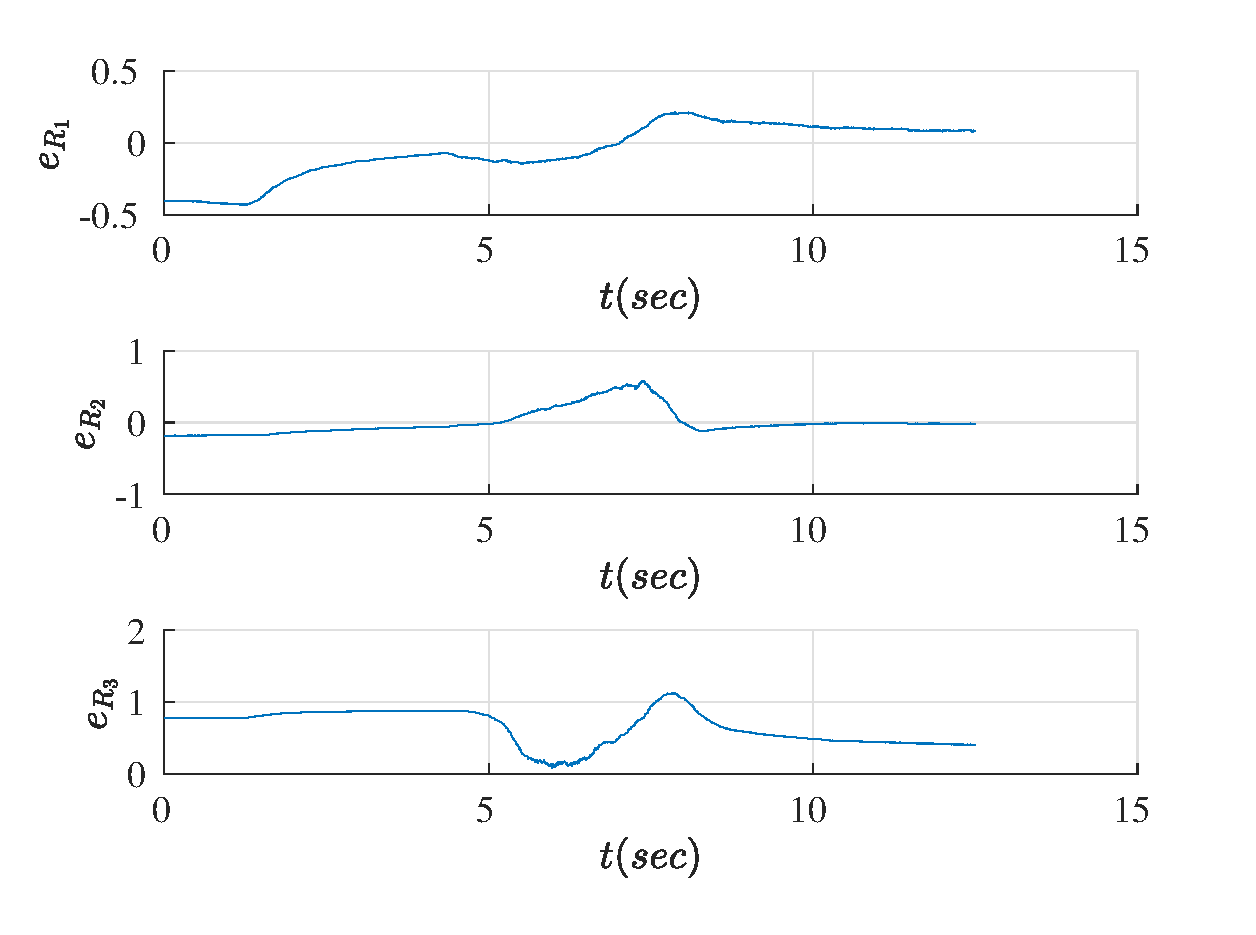
\includegraphics[width=0.5\columnwidth]{eR_exp}  }~
-	\subfigure[{Configuration error \( \Psi \)} \label{fig:Psi_exp} ]{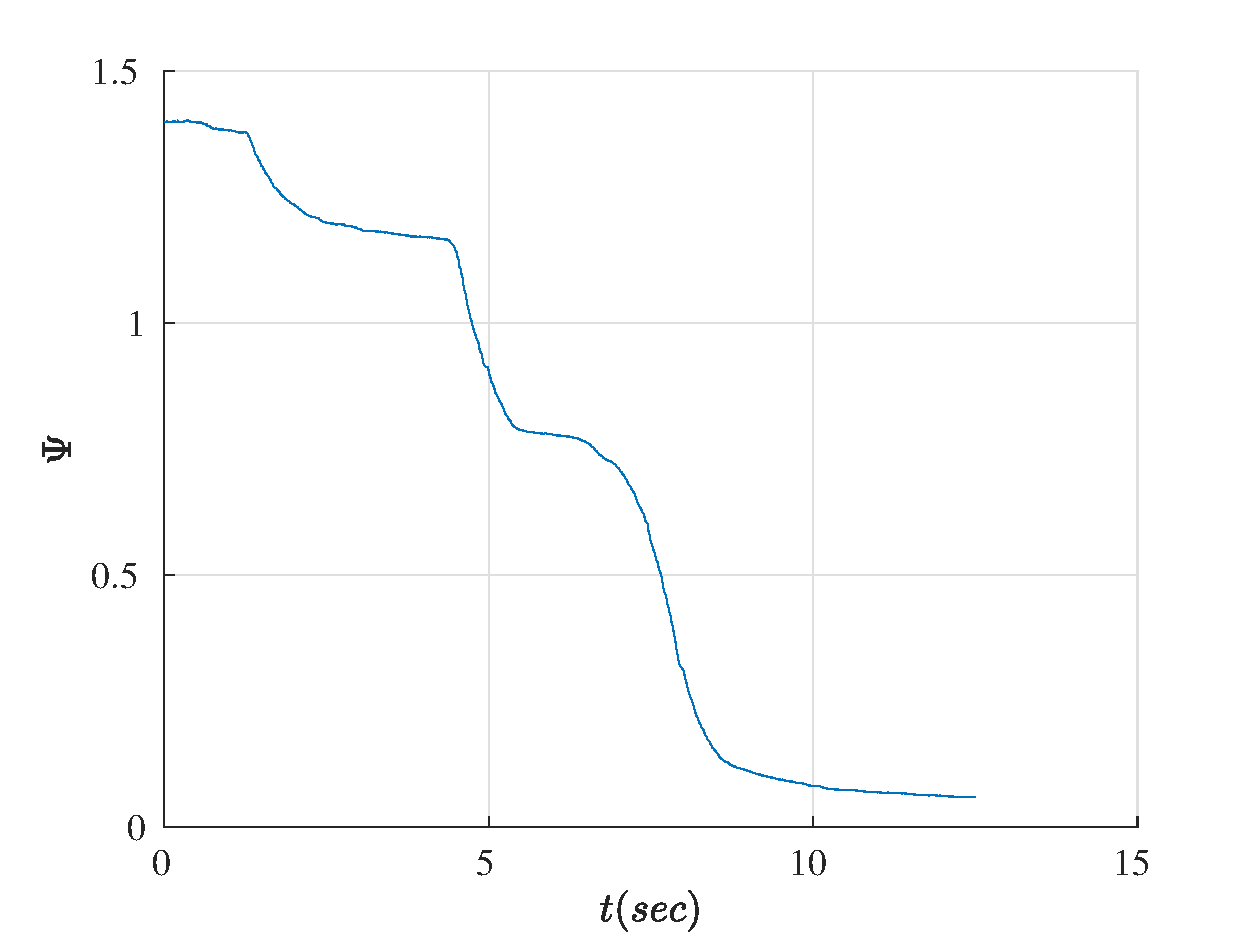
\includegraphics[width=0.5\columnwidth]{Psi_exp} }\\
-	\subfigure[{Control input \( u\) }\label{fig:u_exp}]{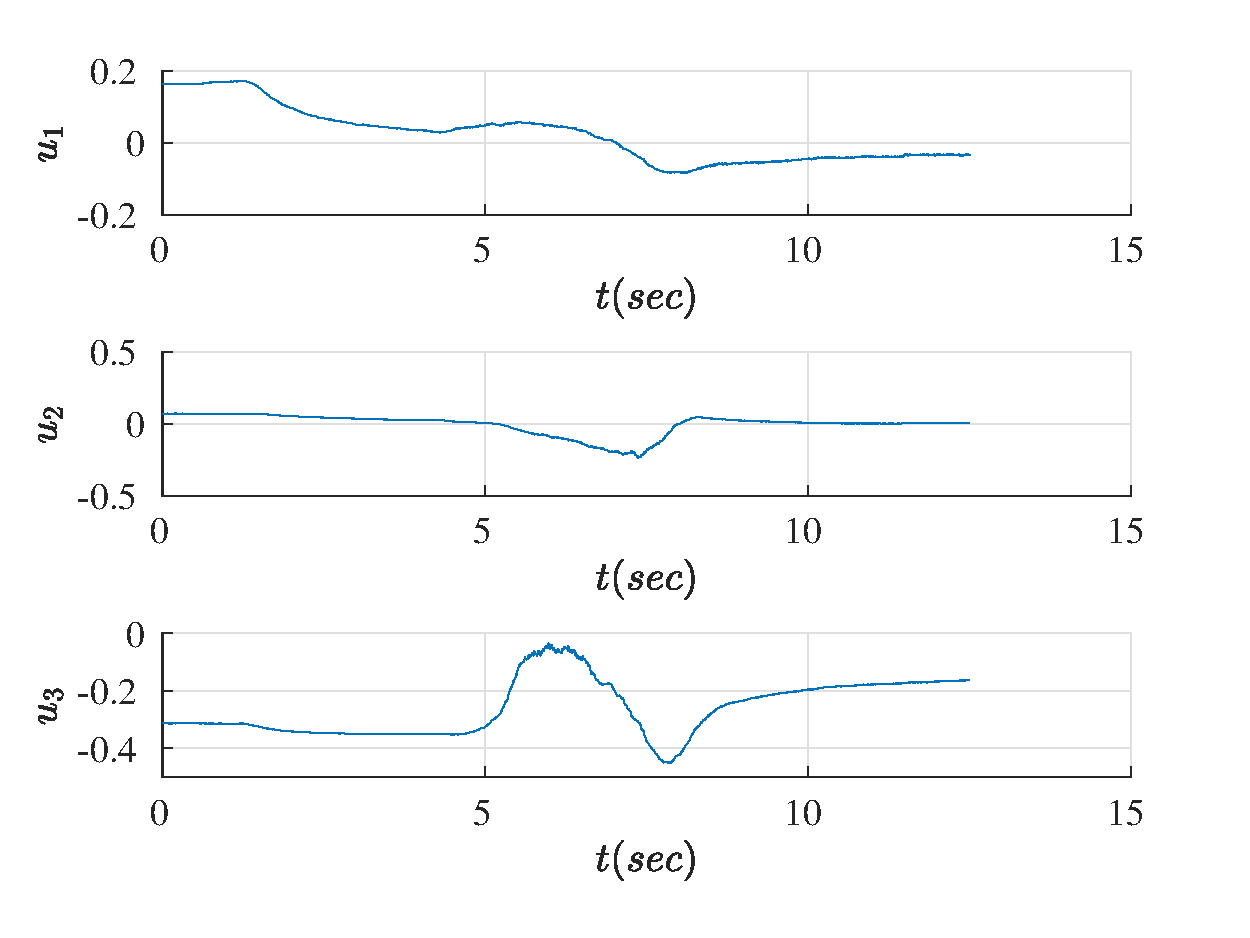
\includegraphics[width=0.5\columnwidth]{u_exp}  }~
-	\subfigure[{Attitude Trajectory } \label{fig:traj_exp}]{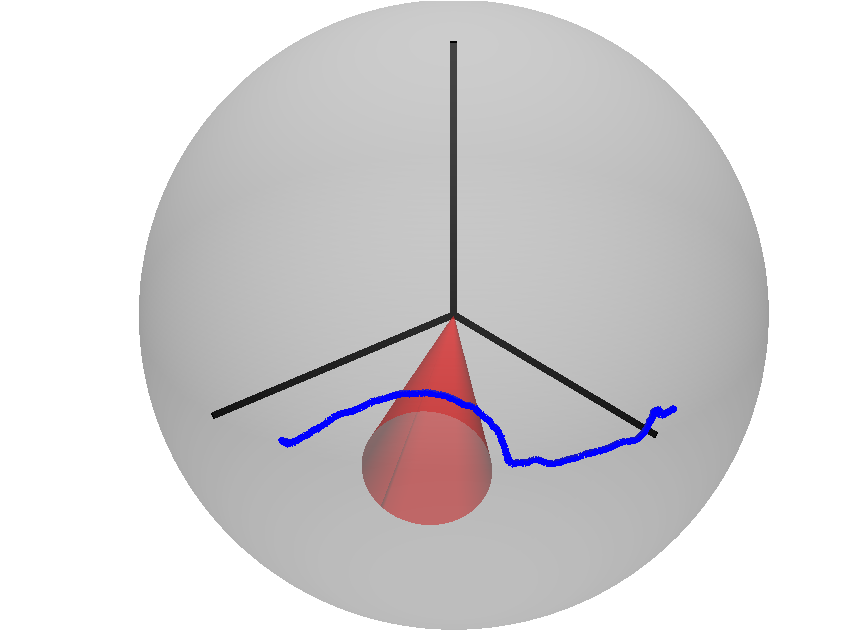
\includegraphics[width=0.5\columnwidth]{traj_exp} }\\
-    \subfigure[{Angle to constraint } \label{fig:con_angle_exp}]{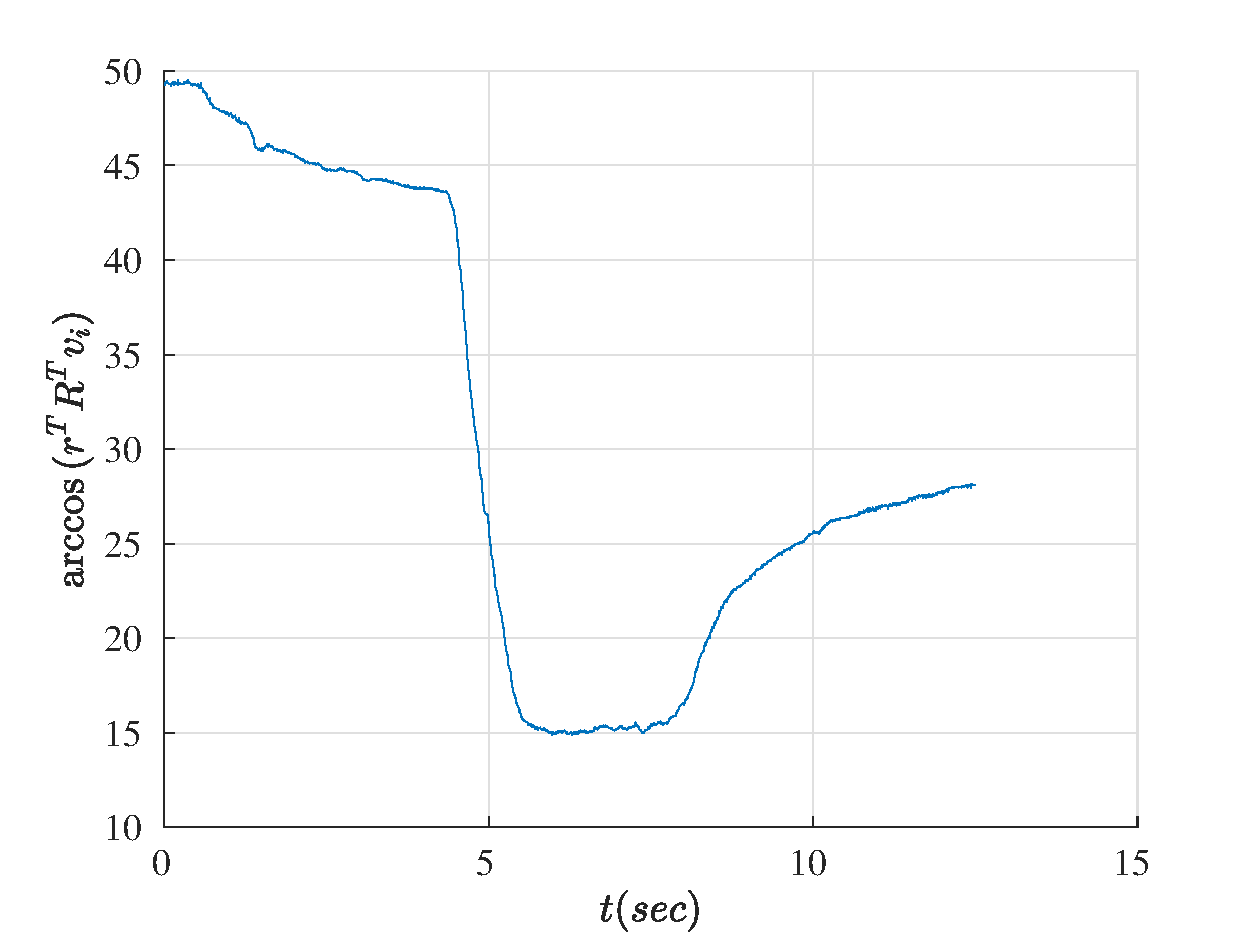
\includegraphics[width=0.5\columnwidth]{figures/constraint_angles_exp.pdf} }
-	\caption{Constrained Attitude stabilization experiment}
-	\label{fig:exp} 
-\end{figure}
+The attitude control system is identical to the one presented in~\Cref{prop:adaptive_control} with the exception of a gravity moment term, \( M_g = r_{cg} \times m g R^T e_3\) which represents the gravitational moment due to the difference between the center of mass and the center of rotation. 
+In addition, the following parameters were also modified: \(k_R = 0.4, k_\Omega = 0.7 ,c = 0.1 , \alpha = 8 \text{ and } k_\Delta = 0.05\) to account for the differences in the hardware model of the hexrotor.
+
 The experimental results are shown in~\Cref{fig:exp}.
+\Cref{fig:eR_exp} shows the behavior of each of the components of the attitude error vector, defined by~\cref{eqn:eR}, over the experiment time span.
+\Cref{fig:Psi_exp} shows the time history of the attitude error function, defined by~\cref{eqn:psi}.
+\Cref{fig:u_exp} shows the magnitude of each component of the control input in \si{\newton\meter}, which is computed from~\cref{eqn:adaptive_control}.
+Finally,~\cref{fig:con_angle_exp} shows the angle between the body-fixed sensor and the obstacle in degrees.
 In order to maneuver the system ``close" to the constrained zone we utilize several intermediary set points on either side of the obstacle.
 From the initial attitude the hexrotor rotates to the first set point, pauses, and then continues around the obstacle to the second set point before continuing toward the desired attitude.
 As a result this creates the stepped behavior of the configuration error history as shown in~\cref{fig:Psi_exp}.
 
+\end{multicols}
+\begin{figure}[H]
+    \centering 
+    \subfigure[{Attitude error vector \(e_R\)} components\label{fig:eR_exp}]{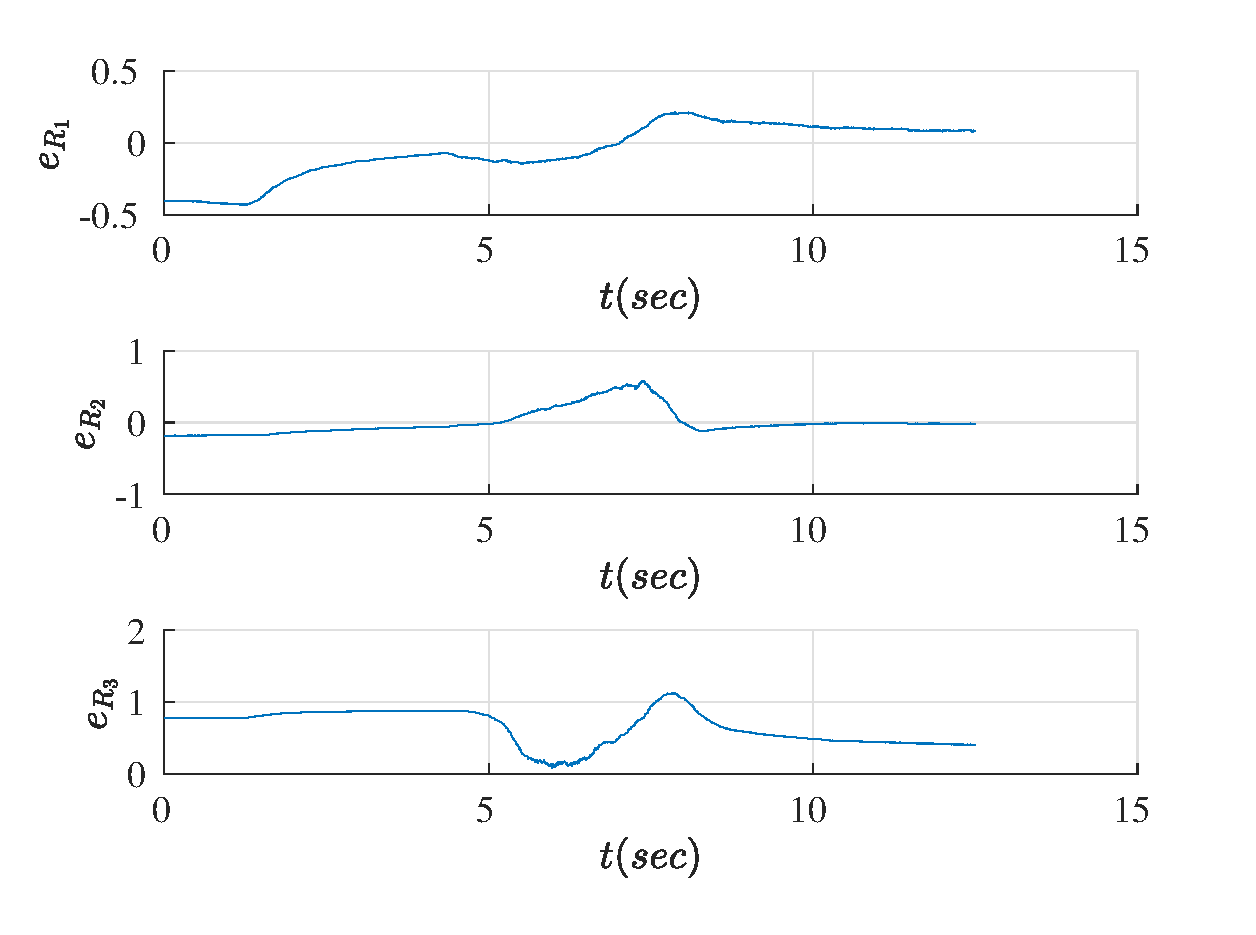
\includegraphics[width=0.3\columnwidth]{eR_exp}  }~
+    \subfigure[{Configuration error \( \Psi \)} \label{fig:Psi_exp} ]{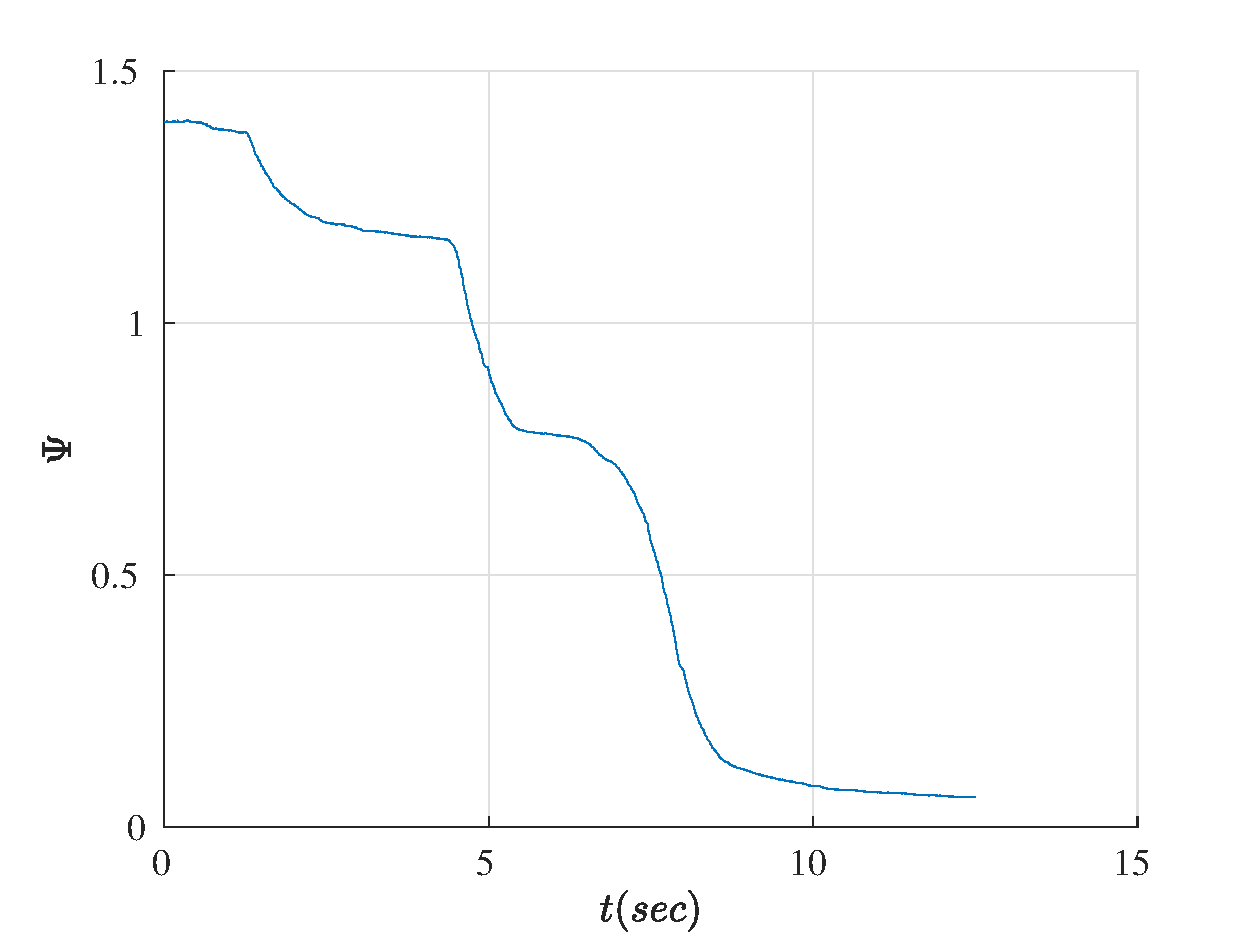
\includegraphics[width=0.3\columnwidth]{Psi_exp} }~
+    \subfigure[{Control input \( u\) } components\label{fig:u_exp}]{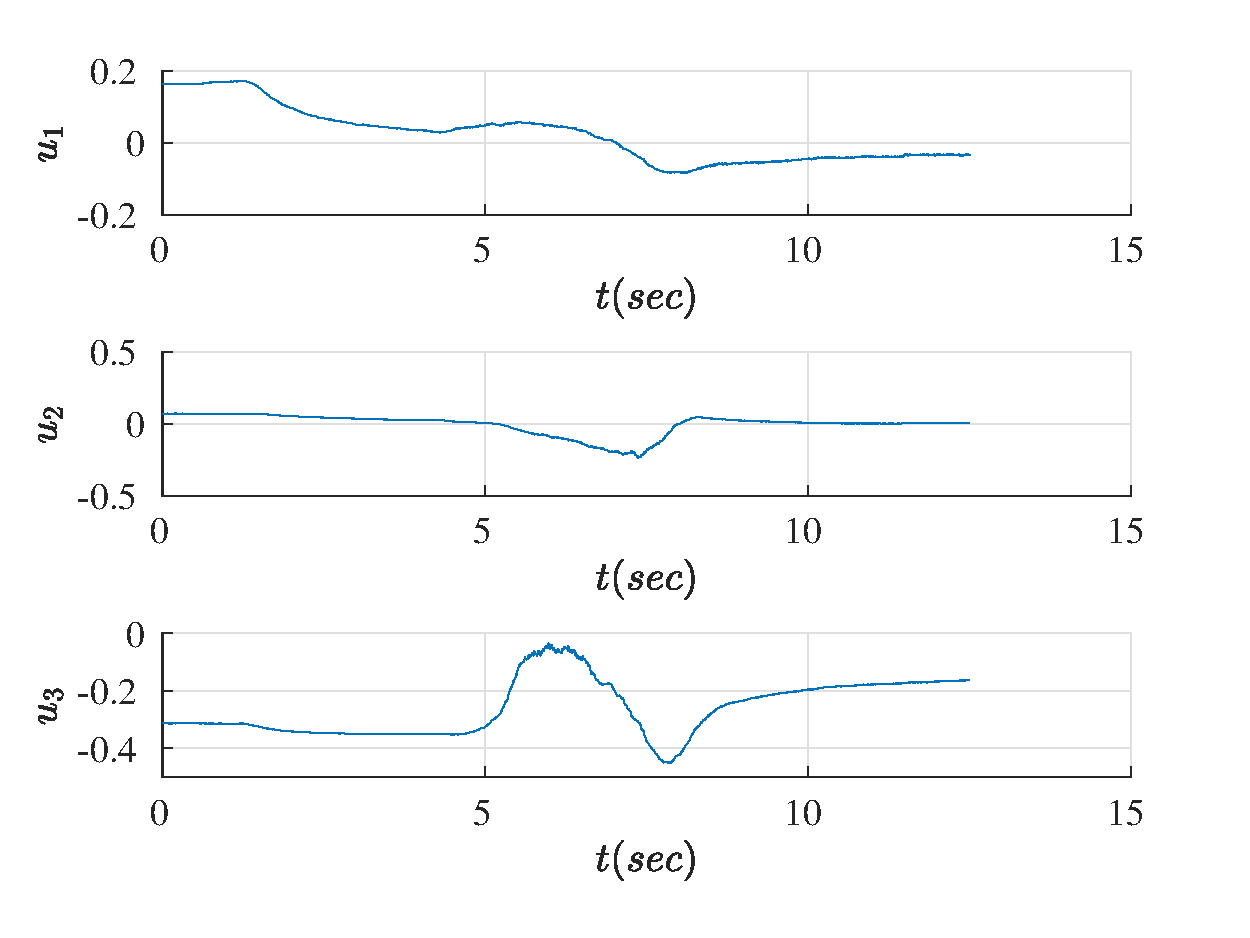
\includegraphics[width=0.3\columnwidth]{u_exp}  }\\
+    \subfigure[{Attitude Trajectory } \label{fig:traj_exp}]{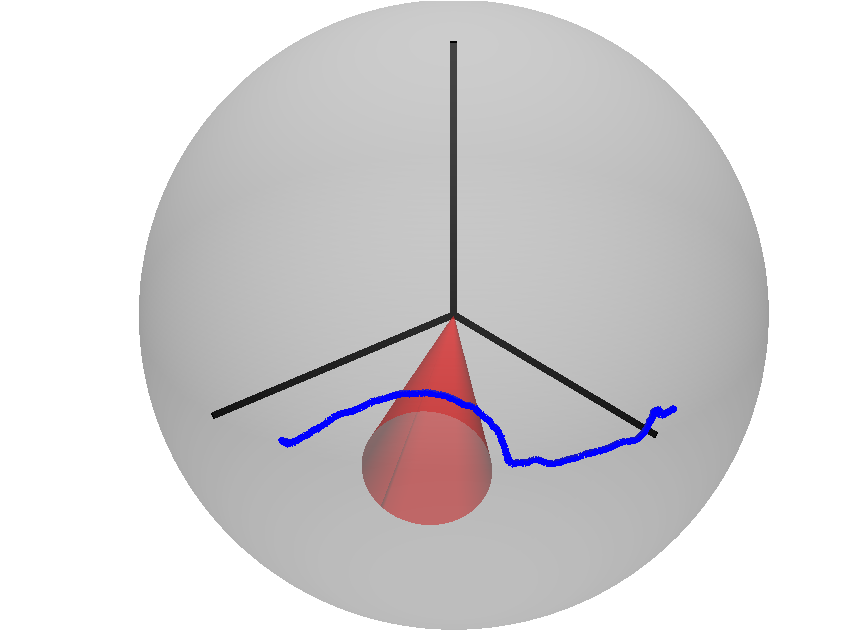
\includegraphics[width=0.3\columnwidth]{traj_exp} }~
+    \subfigure[{Angle to constraint } \label{fig:con_angle_exp}]{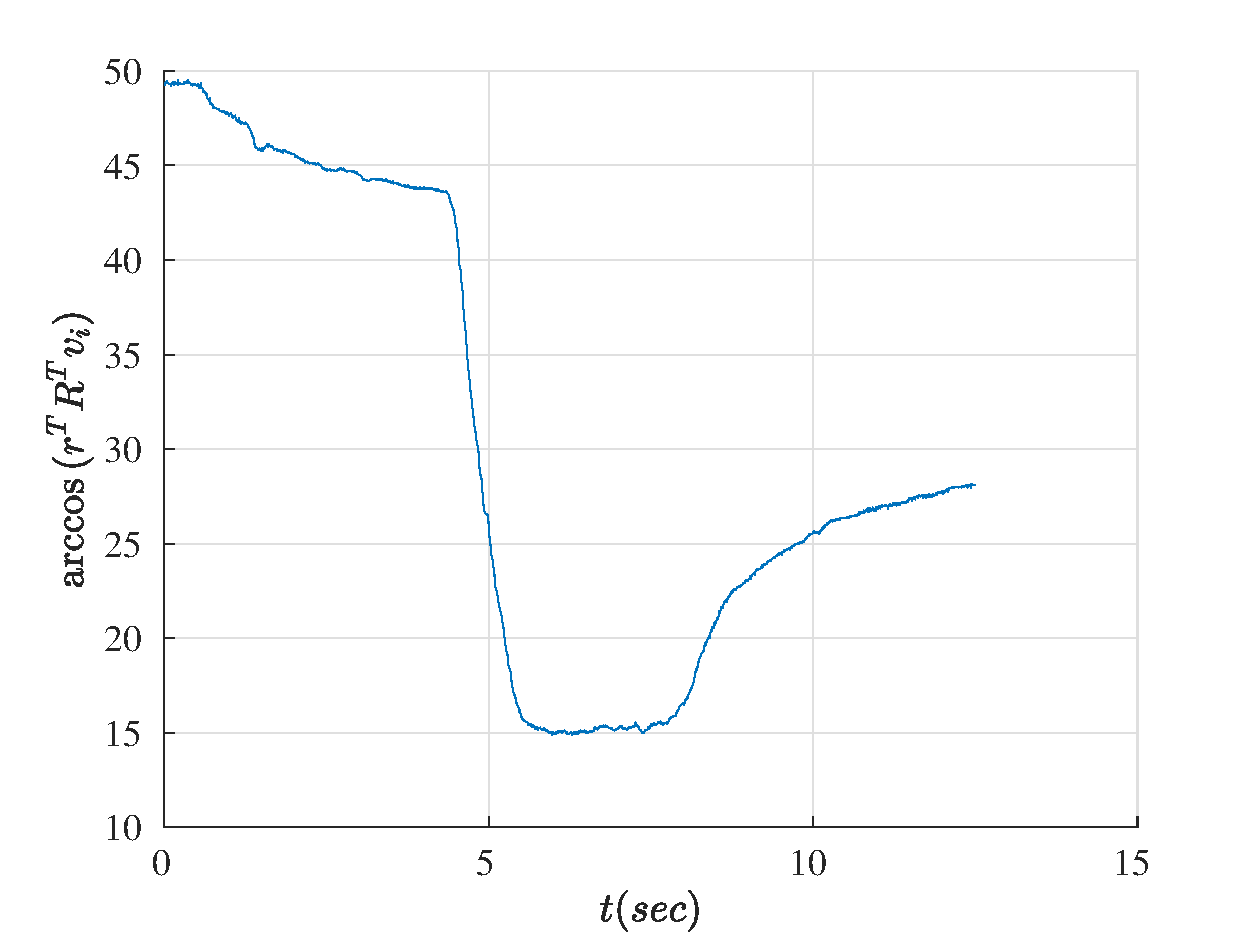
\includegraphics[width=0.3\columnwidth]{figures/constraint_angles_exp.pdf} }
+    \caption{Constrained Attitude stabilization experiment}
+    \label{fig:exp} 
+\end{figure}
+\begin{multicols}{2}
 The hexrotor avoids the constrained region illustrated by the circular cone in~\cref{fig:traj_exp}, by rotating around the boundary of the constraint. 
 \Cref{fig:con_angle_exp} shows the angle, \( \arccos r^T R^T v \), between the body mounted sensor and the inertially fixed sensor.
 The experiment demonstrates that the minimum angular separation is \SI{14}{\degree} which satisfies the constraint of \( \theta = \SI{12}{\degree} \).
 This further validates that the proposed control system exhibits the desired performance in the experimental setting as well. 
-A video clip showing the attitude maneuver is available \url{https://youtu.be/dsmAbwQram4}.
+A video clip is available at \url{https://youtu.be/dsmAbwQram4}.
 
 \section{Conclusions}\label{sec:conclusions}
 We have developed a geometric adaptive control system which incorporates state inequality constraints on \(\SO\).
@@ -560,12 +693,16 @@ As a result, its negative logarithm is always positive and from~\cref{eqn:B}, \(
 The error function \( \Psi = A B \) is composed of two positive terms and is therefore also positive definite.
 
 Next, we consider~\cref{item:prop_era}.
-The variation of~\cref{eqn:A} is taken with respect to \( \delta R = R \hat \eta \) as
+The infinitesimal variation of a rotation matrix is defined as
+\begin{align*}
+    \delta R = \left. \diff{}{\epsilon} \right|_{\epsilon=0} R \exp{\epsilon \hat{\eta}} = R \hat{\eta} .
+\end{align*}
+Using this, the variation of~\cref{eqn:A} is taken with respect to \( R \) as
 \begin{align*}
 	\dirDiff{A}{R} &= \eta \cdot \frac{1}{2} \left( G R_d^T R - R^T R_d G\right)^\vee ,
 %	&= -\frac{1}{2} \tr{G R_d^T \left( R \hat{\eta}\right)} \\
 \end{align*}
-where we used~\cref{eqn:hat1}.
+where we used~\cref{eqn:hat1} to achieve the simplified form.
 
 A straightforward application of the chain and product rules of differentiation allows us to show~\cref{item:prop_erb} as
 \begin{align*}
@@ -580,12 +717,57 @@ where the scalar triple product~\cref{eqn:STP} was used.
 %  A(R) \geq A(R_d) \; \forall \; R \in U .
 %\end{align*}
 %Since the desired attitude, \( R_d \), must lie in the feasible set, i.e., \( r^T R^T v < \cos \theta \), the addition of the repulsive barrier function, \( B \), does not change the minimum value of \( \Psi \).
+We show~\cref{item:prop_psi_quadratic} by computing the hessian of \( \Psi \), namely \( \Hess(\Psi) \),  using the chain rule as 
+\begin{align*}
+    \Hess &(\Psi)\cdot (\delta R,\delta R)= (\mathbf{D}_R\parenth{\mathbf{D}_R A \cdot \delta R}\cdot \delta R) B\\
+    & + \parenth{\dirDiff{A}{R} }\parenth{\dirDiff{B}{R}} 
+    + \parenth{\dirDiff{B}{R} }\parenth{\dirDiff{A}{R}}\\ &+(\mathbf{D}_R\parenth{\mathbf{D}_R B \cdot \delta R}\cdot \delta R) A.
+\end{align*}
+The first order derivative of \( A(R) \) and \( B(R) \) are given by~\cref{eqn:eRA,eqn:eRB}. 
+The hessian of \( A(R) \) is computed as 
+\begin{align*}
+    \dirDiff{\parenth{\dirDiff{A}{R}}}{R} &= \eta \cdot \frac{1}{2}\parenth{G R_d^T \delta R - \delta R^T R_d G}^\vee , \\
+    &= \eta \cdot \frac{1}{2} \parenth{G R_d^T R \hat \eta + \hat \eta R^T R_d G}^\vee,\\
+    &= \eta \cdot \frac{1}{2} \bracket{\parenth{\braces{\tr{R^T R_d G} I - R^T R_d G} \eta}^\wedge}^\vee , \\
+    &= \eta \cdot \frac{1}{2} \parenth{\tr{R^T R_d G} I - R^T R_d G}\eta ,
+\end{align*}
+where we used the scalar triple product rule, from~\cref{eqn:STP}, to arrive at the final form.
+The hessian of \( B(R) \) is computed as
+\begin{align*}
+    \dirDiff{\parenth{\dirDiff{B}{R}}}{R} =& \eta \cdot \left[\frac{\parenth{\delta R^T v}^\wedge r}{\alpha\parenth{r^T R^T v - \cos \theta}} \right. \\
+    & \left. - \frac{\parenth{R^T v}^\wedge r \parenth{r^T \delta R^T v}}{\alpha \parenth{r^TR^Tv - \cos \theta}^2}   \right] .
+\end{align*}
+The term \( \parenth{\delta R^T v}^\wedge r\) is simplified as
+\begin{align*}
+    \parenth{\delta R^T v}^\wedge r &= - \hat{r} \delta R ^T v , \\
+    &= - \hat{r} \parenth{R \hat \eta}^T v , \\
+    &= \hat{r} \parenth{\hat{\eta} R^T } v , \\
+    &= - \hat{r} \parenth{R^T v}^\wedge \eta ,
+\end{align*}
+where we utilized the hat map property from~\cref{eqn:cross_product}.
+Similarly, the term \( r^T \delta R^T v \) is simplified as
+\begin{align*}
+    r^T \delta R^T v &= r^T \parenth{-\hat \eta R^T}v , \\
+    &= r^T \parenth{R^T v}^\wedge \eta .
+\end{align*}
+The hessian of \( B(R) \) then becomes
+\begin{align*}
+    \dirDiff{\parenth{\dirDiff{B}{R}}}{R} =& \eta \cdot \left[ - \frac{ \hat r \parenth{R^T v}^\wedge}{\alpha \parenth{r^T R^T v - \cos \theta}} \right. \\ 
+    & \left. - \frac{\parenth{R^T v}^\wedge r r^T \parenth{R^T v}^\wedge }{ \alpha\parenth{r^T R^T v - \cos \theta}^2}  \right] \eta .
+\end{align*}
+Using these terms, we evaluate \( \Hess{\Psi} \) at the desired attitude \( R = R_d \) as follows. Since $A=0$ and $\mathbf{D}_R A=0$ at $R=R_d$, 
+\begin{align*}
+    \Hess(\Psi)\cdot (\delta R,\delta R)\big|_{R=R_d} = \eta \cdot \frac{1}{2} B \parenth{\tr{G}I -  G} \eta , 
+\end{align*}
+which is positive definite since \( B > 1\) and \( \sum g_i > g_i\). 
+The domain \( D \) is an open neighborhood of the desired attitude \( R_d \), and it excludes the undesired equilibrium points of \( A(R) \) and the infeasible regions defined by the constraints \( r^T R^T v_i \). 
+Therefore, the only critical point of the error function $\Psi$ in the domain $D$ corresponds to the desired attitude $R=R_d$ with $e_R=0$ and $\Psi=0$. 
+Therefore, in \( D \) the configuration error function is quadratic and the bounds in~\cref{item:prop_psi_quadratic} are valid according to~\cite[Proposition 6.30]{bullo2004}.
 
-The desired equilibrium occurs at \( R=R_d\) and results in \( e_R = 0 \) and \( \Psi = A = 0\).
 The proof of \cref{item:prop_era_upbound} is available in~\cite{LeeITCST13}.
 
 \subsection{Proof of~\Cref{prop:error_dyn}}\label{proof:error_dyn}
-From the kinematics~\cref{eqn:Rdot} and noting that \( \dot{R}_d = 0 \) the time derivative of \( R_d^T R \) is given as
+From the kinematics~\cref{eqn:Rdot}, and noting that \( \dot{R}_d = 0 \) the time derivative of \( R_d^T R \) is given as
 \begin{gather*}
 	\diff{}{t} \parenth{R_d^T R} = R_d^T R \hat{e}_\Omega .
 \end{gather*}
@@ -659,11 +841,18 @@ Therefore, the inequality constraint is always satisfied given that the desired
 %	We assume that \( B > \psi \) which implies that \( A < 1 \).
 %	As \( \psi \) is increased this implies that the system is approaching the constraint and that \( A \to 0 \) in order to remain in the domain \( D \).
 %	However, since the chosen domain is assumed to exclude the constraint this situation is not possible and \( B < \psi \).
+%We choose the domain \( D \) to exclude the undesired critical points of \( A(R) \) as well as the infeasible regions defined by the state inequality constraints. 
+%Furthermore,~\cref{proof:config_error} shows that \(D \) is an open neighborhood of the desired attitude configuration, \( R_d\).
+%The proof of the upper bound of \( A(R) \) is given in~\cite{LeeITCST13}.
+
+
+Consider the open neighborhood $D$ of $R=R_d$ defined in~\Cref{prop:config_error}.
+The proof of the upper bound of \( A(R) \) is given in~\cite{LeeITCST13}.
 The selected domain ensures that the configuration error function is bounded \( \Psi < \psi \).
 This implies that that both \( A(R) \) and \( B(R) \) are bounded by constants \( c_A c_B < \psi < h_1\).
 Furthermore, since \( \norm{B} > 1 \) this ensures that \( c_A, c_B < \psi\) and shows~\cref{eqn:AB_bound}.
 
-Next, we show~~\cref{eqn:E_bound,eqn:F_bound} using the Frobenius norm.
+Next, we show~\cref{eqn:E_bound,eqn:F_bound} using the Frobenius norm.
 The Frobenius norm \( \norm{E}_F \) is given in~\cite{LeeITCST13} as
 \begin{gather*}
 	\norm{E}_F = \sqrt{\tr{E^T E}} = \frac{1}{2} \sqrt{\tr{G^2} + \tr{R^T R_d G}^2} .
@@ -724,22 +913,35 @@ Using~\crefrange{eqn:AB_bound}{eqn:eRB_bound} one can define \( H \) in terms of
 \subsection{Proof of~\Cref{prop:adaptive_control}}\label{proof:adaptive_control}
 Consider the Lyapunov function \( \mathcal{V} \) given by
 \begin{align*}
-	\mathcal{V} = \frac{1}{2} e_\Omega \cdot J e_\Omega + k_R \Psi + c J e_\Omega \cdot e_R + \frac{1}{2 k_\Delta} e_\Delta \cdot e_\Delta , \label{eqn:v_adapt}
+	\mathcal{V} = \frac{1}{2} e_\Omega \cdot J e_\Omega + k_R \Psi + c J e_\Omega \cdot e_R + \frac{1}{2 k_\Delta} e_\Delta \cdot e_\Delta , %\label{eqn:v_adapt}
 \end{align*}
-over the domain \( D \) in~\cref{eqn:domain}.
-From~\Cref{prop:eR_dot_bound}, the Lyapunov function is bounded in \( D \) by
+over the domain \( D \), defined in~\cref{prop:config_error}. 
+In this set, the properties of~\Cref{prop:config_error,prop:error_dyn} are satisfied.
+%Furthermore, the set \( D \) is an open neighborhood of the desired attitude and Lyapunov stability results are valid in this set.
+
+From~\Cref{prop:config_error}, the configuration error function is locally quadratic and it is bounded in \( D \) by~\cref{eq:psi_bound}.
+Using this, the Lyapunov function \( \mathcal{V} \) is bounded by
 \begin{align*} %\label{eqn:v_upper_bound}
-	\mathcal{V} \leq z^T W z ,
+	z^T W_1 z \leq \mathcal{V} \leq z^T W_2 z ,
 \end{align*}
-where \( e_\Delta = \Delta - \bar{\Delta} \), \( z = [\|e_R\|,\|e_\Omega\|,\|e_\Delta\|]^T\in\R^3 \) and the matrix \(W \in \R^{3 \times 3}\) is given by
-\begin{gather*}
-	W = \begin{bmatrix}
-		k_R \psi & \frac{1}{2} c \lambda_M & 0 \\
+where \( e_\Delta = \Delta - \bar{\Delta} \), \( z = [\|e_R\|,\|e_\Omega\|,\|e_\Delta\|]^T\in\R^3 \) and the matrices \(W_1,W_2 \in \R^{3 \times 3}\) are given by
+\begin{align*}
+	W_1 & = \begin{bmatrix}
+		k_R n_1 & -\frac{1}{2} c \lambda_M & 0 \\
+		-\frac{1}{2} c \lambda_M & \frac{1}{2} \lambda_m & 0 \\
+		0 & 0 & \frac{1}{2 k_\Delta}
+	\end{bmatrix},\\
+	W_2 & = \begin{bmatrix}
+		k_R n_2 & \frac{1}{2} c \lambda_M & 0 \\
 		\frac{1}{2} c \lambda_M & \frac{1}{2} \lambda_M & 0 \\
 		0 & 0 & \frac{1}{2 k_\Delta}
 	\end{bmatrix} .
-\end{gather*}
-The time derivative of \( \mathcal{V}\) with the control inputs~\cref{eqn:adaptive_control} is given by
+\end{align*}
+%\begin{gather*}
+%\frac{1}{2}\lambda_m k_R n_1 - \frac{1}{4}c^2 \lambda_M^2 >0\\
+%\frac{2\lambda_m k_R n_1}{\lambda_M^2} > c^2 \\
+%\end{gather*}
+The time derivative of \( \mathcal{V}\) with the control input defined by~\cref{eqn:adaptive_control} is given as
 \begin{align*}
 	\dot{\mathcal{V}} =& - k_\Omega e_\Omega^T e_\Omega + \parenth{e_\Omega + c e_R}^T W e_\Delta - k_R c e_R^T e_R \nonumber\\
 	&- k_\Omega c e_R^T e_\Omega + c J e_\Omega^T \dot{e}_R - \frac{1}{k_\Delta} e_\Delta^T \dot{\bar{\Delta}} , \label{eqn:vdot}
@@ -749,7 +951,7 @@ The terms linearly dependent on \( e_\Delta\) are combined with~\cref{eqn:delta_
 \begin{align*}
 	 e_\Delta^T \parenth{W^T \parenth{e_\Omega + c e_R} - \frac{1}{k_\Delta} \dot{\bar{\Delta}}} = 0 . 
 \end{align*}
-Using~\Cref{prop:eR_dot_bound} an upper bound on \( \dot{\mathcal{V}} \) is written as
+Using~\Cref{prop:eR_dot_bound}, an upper bound on \( \dot{\mathcal{V}} \) is written as
 \begin{gather*}
 	\dot{\mathcal{V}} \leq -\zeta^T M \zeta ,
 \end{gather*}
@@ -760,9 +962,17 @@ where $\zeta=[\|e_R\|,\|e_\Omega\|]\in\R^2$, and the matrix \( M \in \R^{2 \time
 		\frac{k_\Omega c}{2} & k_\Omega - c \lambda_M H
 	\end{bmatrix} .
 \end{gather*}
-If \( c \) is chosen such that~\cref{eqn:c_bound} is satisfied the matrix \( M \) is positive definite.
-This implies that $\dot{\mathcal{V}}$ is negative semidefinite and $\lim_{t\to\infty} \zeta=0$. 
-As the Lyapunov function is non-increasing $z$ is uniformly bounded. 
+%\begin{gather*}
+%k_R c (k_\Omega -c \lambda_M H) -\frac{1}{4}k_\Omega^2 c^2 < 0\\
+%k_R (k_\Omega -c \lambda_M H) -\frac{1}{4}k_\Omega^2 c < 0\\
+%4k_R k_\Omega -c(4k_R \lambda_M H +k_\Omega^2) <0
+%\end{gather*}
+
+If \( c \) is chosen such that~\cref{eqn:c_bound} is satisfied then the matrices \( W_1, W_2 \) and \( M \) are positive definite.
+This implies that $\mathcal{V}$ is positive definite and decrescent, and $\dot{\mathcal{V}}$ is negative semidefinite in the domain $D$. As such, the zero equilibrium is stable in the sense of Lyapunov, and all of the error variables are bounded. Furthermore, $\lim_{t\to\infty} \zeta=0$ according to the LaShalle-Yoshizawa theorem~\cite{khalil1996}. 
+
+%and 
+%As the Lyapunov function is non-increasing $z$ is uniformly bounded. 
 %	
 %	
 %	This implies that the Lyapunov function \( V \) is non-increasing and bounded from below.
@@ -771,30 +981,22 @@ As the Lyapunov function is non-increasing $z$ is uniformly bounded.
 %	The domain \( D \) does that include the undesired equilibria and ensures that as \( e_R \to 0 \) the attitude also converges \( R \to R_d \).
 %%%%%%%%%%%%%%%%%%%%%%%%%%%%%%%%%%%%%%%%%%%%%%%%%%%%%%%%%%%%%%%%%%%%%%%%%%%%%%%%
 
-%\addtolength{\textheight}{-12cm}   % This command serves to balance the column lengths
-                                  % on the last page of the document manually. It shortens
-                                  % the textheight of the last page by a suitable amount.
-                                  % This command does not take effect until the next page
-                                  % so it should come on the page before the last. Make
-                                  % sure that you do not shorten the textheight too much.
-                                  
 \bibliography{BibMaster,library}
 \bibliographystyle{IEEEtran}
-
 \biography{profile}{Shankar Kulumani}
     {is a PhD Candidate in the Department of Mechanical and Aerospace Engineering at George Washington University. 
-    He received his bachelor's degree in Astronautical Engineering from the United States Air Force Academy in 2009 and his master's in Aeronautical and Astronautical Engineering from Purdue University in 2013.
+    He received his bachelor's degree in Astronautical Engineering from the US Air Force Academy in 2009 and his master's degree in Aeronautical and Astronautical Engineering from Purdue University in 2013.
     % He previously served as Deputy Space Vehicles Lead for the ORS-1 (Operationally Responsive Space ) satellite program, and as Lead Test Engineer in the Guidance, Navigation, and Control group at Air Force Research Laboratory located at Kirtland AFB, NM.
     % He is now currently a reserve air force officer where he serves as Threat Systems Engineer for the Missle and Space Intelligence Center, Defense Intelligence Agency.
     His current research interests include the application of geometric mechanics and control to aerospace systems. 
     }
-
 \biography{Lee}{Taeyoung Lee}
     {is an associate professor of Department of Mechanical and Aerospace Engineering at the George Washington University. 
     He received his doctoral degree in Aerospace Engineering and his master's degree in Mathematics at the University of Michigan in 2008. 
     His research interests include computational geometric mechanics and control of complex systems.}    
 \clearafterbiography\relax
 \clearafterbiography\relax
+
 \end{multicols}
 
 \end{document}
